\documentclass[a4paper]{article}

\usepackage{pdp}
\usepackage{float}

%------------------------------------------------------------------------------
% REPORT INFORMATION
%-----------------------------------------------nombreu-------------------------------

\title{Othello -- Python}
\subtitle{Rapport final}
\author{Grégory Bonzon, Rémi Boussion, Gabriel Ringuet, Matthieu Vigier-Lafosse, Arthur Voisin}

%------------------------------------------------------------------------------

\begin{document}

%------------------------------------------------------------------------------
% TITLE PAGE
%------------------------------------------------------------------------------

\maketitle
\thispagestyle{empty}

%------------------------------------------------------------------------------
% MAIN MATTER
%------------------------------------------------------------------------------

\section{Explication Détaillée du Sujet}
\subsection{Historique du Jeu}

L'Othello, également connu sous le nom de Reversi, est un jeu de stratégie abstrait
qui possède une riche histoire. Il a été inventé au 19ème siècle en Angleterre,
avant que son format actuel ne se répande au Japon au cours du 20ème siècle pour
finalement devenir un jeu mondialement pratiqué \cite{WOF}. L'attrait global pour ce jeu
se manifeste notamment par l'organisation de championnats du monde annuels depuis 1977 \cite{WOF}.
Sur le plan informatique, l'Othello a longtemps représenté un défi majeur pour l'intelligence
artificielle \cite{Rosenbloom1982,Lee1990,Buro1997} en raison de son immense espace d'exploration, estimé à $10^{58}$ de parties
possibles et $10^{28}$ de positions de plateau \cite{Takizawa2024}.

Ce n'est que très récemment, en 2024, que le jeu a été "résolu" de manière faible
("weakly solved")\cite{Takizawa2024}. Il a ainsi été prouvé informatiquement qu'une partie jouée parfaitement
par les deux joueurs aboutit inévitablement à un match nul \cite{Takizawa2024}.

\subsection{Règles du Jeu}

L'Othello est un jeu de plateau à information parfaite et déterministe conçu pour deux joueurs \cite{OthelloSpecs2025}.
Les règles fondamentales régissant les parties sont les suivantes :
Le jeu oppose le joueur Noir au joueur Blanc, et c'est le joueur Noir qui joue le premier coup \cite{WOF}.
Les joueurs jouent ensuite à tour de rôle. La taille classique du plateau est de 8 cases par 8 \cite{OthelloSpecs2025}.


Un joueur a l'obligation de poser une pièce sur une case vide de manière à encadrer une
ou plusieurs pièces adverses en ligne droite (horizontalement, verticalement ou diagonalement)
entre la nouvelle pièce et une pièce déjà existante à sa couleur \cite{WOF}. Les pièces adverses ainsi
encadrées sont alors retournées pour prendre la couleur du joueur ayant joué.

\begin{figure}[H]
    \centering
    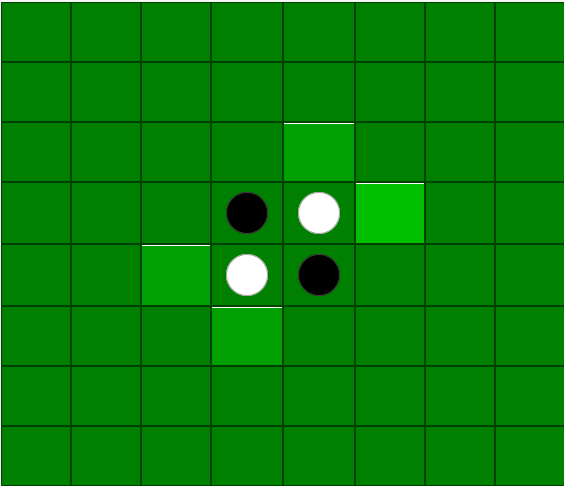
\includegraphics[width=0.3\textwidth]{images/config-init.png}
    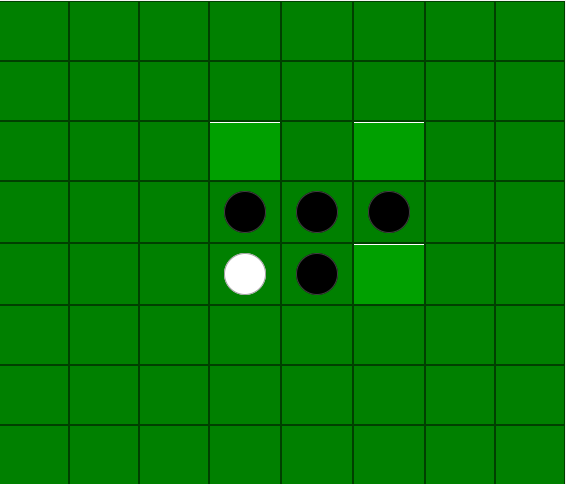
\includegraphics[width=0.3\textwidth]{images/retournement.png}
    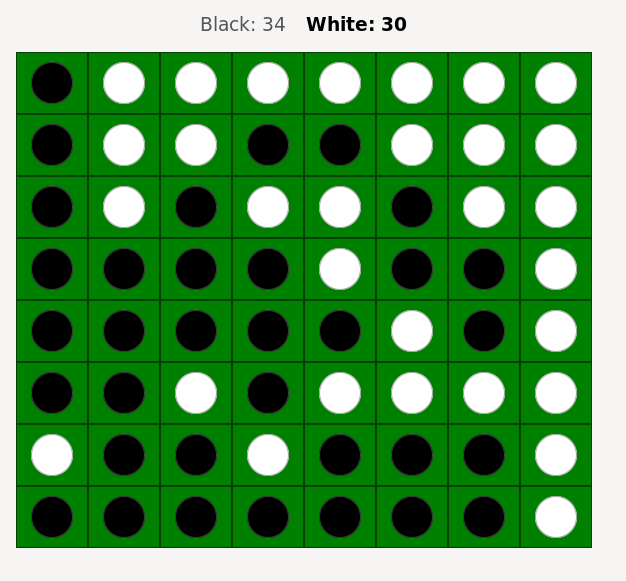
\includegraphics[width=0.3\textwidth]{images/fin_partie.png}
    \caption{Configuration initiale, retournement d'un pion et position finale.}
\end{figure}


Un joueur ne peut placer une pièce que si ce coup permet de retourner au moins une pièce adverse \cite{WOF}.
Si aucun coup légal n'est possible, le joueur doit passer son tour. La partie s'arrête lorsque
le plateau est entièrement rempli ou lorsqu'aucun des deux joueurs ne peut plus poser de pièce.
Le vainqueur est celui qui possède le plus grand nombre de pièces de sa couleur sur le plateau
à la fin de la partie.

\subsection{L'existant et Positionnement du Projet}
Il existe aujourd'hui de nombreux logiciels d'Othello très performants, à l'image du programme
Edax \cite{Edax2023}, qui utilise des algorithmes de recherche de type alpha-bêta très optimisés pour le jeu
à haut niveau \cite{Takizawa2024}.

Notre projet vise à reproduire un écosystème logiciel complet autour du jeu,
développé en Python (version 3.10+) \cite{OthelloSpecs2025, Python310}. Contrairement à de simples implémentations des règles,
notre logiciel se démarque par une architecture robuste intégrant : Une représentation de l'état
du jeu par des "bitboards", permettant de manipuler le plateau via des opérations binaires
extrêmement rapides \cite{Browne2014}. Une double interface : une interface en ligne de commande (CLI) sous forme
de shell interactif et une interface graphique (GUI) développée avec PyGObject. Plusieurs
intelligences artificielles implémentant l'algorithme Minimax avec élagage alpha-bêta ainsi
qu'une recherche arborescente Monte Carlo (MCTS) \cite{Browne2012}. Des fonctionnalités avancées comme le jeu en
réseau client-serveur et le support de plateaux de tailles variables (6x6, 8x8, 10x10, 12x12) \cite{OthelloSpecs2025}.

\section{Algorithmes et Structures de Données}
\subsection{Implémentation des Bitboards}
L'état du jeu est stocké de manière hautement optimisée à l'aide de bitboards gérés au sein de la classe \texttt{GameState}.

\begin{figure}[H]
    \centering
    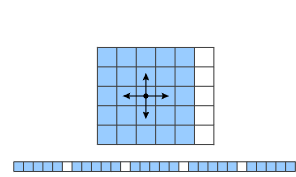
\includegraphics[width=0.4\textwidth]{images/CorrespondanceBB.png}
    \caption{Un plateau de 5×5 avec des bits de séparation dans la colonne de droite et son masque (Source : \cite{Browne2014}).}
\end{figure}
La représentation binaire encode le plateau sous la forme de deux entiers de 64 bits, \texttt{white\_board} et \texttt{black\_board}, où chaque bit représente l'état d'une case \cite{Browne2014}. Cette gestion est rendue dynamique par le module \texttt{BitboardOps} qui recalcule à la volée les masques de plateau (\texttt{FULL\_MASK}) pour supporter des grilles allant de 6x6 jusqu'à 12x12 \cite{OthelloSpecs2025}. De surcroît, afin d'éviter qu'un pion ne passe logiquement d'un bord à l'autre lors des décalages binaires, des masques spécifiques anti-débordement comme \texttt{MASK\_NOT\_A} et \texttt{MASK\_NOT\_H} sont appliqués systématiquement \cite{Browne2014}.

\subsection{Implémentation des Piles}
Pour répondre au besoin d'annulation et de restauration des coups (Undo/Redo), le projet s'appuie sur la structure de données en pile (Stack), implémentée via des listes en Python fonctionnant sur le principe LIFO (Last In, First Out) \cite{Python310}.

La pile d'historique (Undo) sauvegarde systématiquement les coups du joueur en "poussant" (push) l'état complet du jeu précédant l'action au sommet de la pile. Lors d'un "undo", le programme "dépile" (pop) ce dernier élément pour restaurer l'état précédent du plateau. L'action d'annulation transfère également cet état vers la pile de restauration (Redo) pour pouvoir rejouer le coup annulé. Cependant, il est impératif d'assurer la cohérence de la nouvelle branche de jeu : ainsi, si un joueur joue de lui-même un tout nouveau coup suite à un ou plusieurs "undo", il se produit un écrasement du futur, et la pile de "redo" est entièrement vidée du contexte obsolète.

\subsection{Algorithmes Spécifiques au Moteur de Jeu}
Les règles du jeu (\texttt{GameRules}) s'appuient sur des opérations logiques (bit à bit) pour déterminer
l'état de la partie instantanément.

L'algorithme de génération de coups (\texttt{get\_legal\_moves}) identifie d'abord les cases vides via l'opération logique \verb+~(player_bb | opponent_bb) & BitboardOps.FULL_MASK+. Il itère ensuite sur les huit directions possibles en décalant les bits du joueur de la distance requise et en appliquant un masquage binaire (\&) strict avec les pions adverses pour isoler les coups valides. 
L'algorithme de retournement (\texttt{compute\_flips}) s'inscrit dans cette suite en propageant l'effet dans les directions ciblées et accumulant un masque de retournement temporaire (\texttt{potential\_flips}). Ce masque n'est validé (et donc fusionné au registre en modification) que s'il rencontre en bout de propagation une pierre de la couleur du joueur courant. L'identification de fin de partie repose sur la capacité de cet ensemble formel à trouver ou non des branches, un état devenant terminal de fait si le plateau est physiquement rempli, ou si les deux joueurs manquent simultanément de mouvements légaux. Le score de cette position d'arrêt est calculé très rapidement via la fonction matérielle de comptage binaire \texttt{popcount} (accessible via \texttt{.bit\_count()}).


\subsection{Algorithmes d'Intelligence Artificielle}
La classe \texttt{AIPlayer} encapsule les algorithmes de décision du joueur artificiel.

Concernant les méthodes classiques, l'implémentation repose conjointement sur la variante Négamax, qui simplifie la gestion de l'alternance des joueurs Max et Min \cite{Knuth1997}, et sur l'élagage alpha-bêta, dont l'avantage est de couper formellement l'exploration des branches sous-optimales de l'arbre et ainsi d'accélérer drastiquement la recherche \cite{Takizawa2024, Knuth1997}. Afin de moduler cette analyse déterministe avec précision chronométrique, l'algorithme procède par approfondissement itératif, l'IA décortiquant les scénarios de plus en plus profondément de façon incrémentale jusqu'à l'interruption exacte sur l'expiration du temps alloué. 
Pour aborder des profils probabilistes d'adversité, le framework tire parti du Monte Carlo Tree Search (MCTS) utilisant notamment la formule UCB1 pour concilier au plus juste la part d'exploration et d'exploitation inhérente lors de ses simulations basées sur le hasard (\textit{rollouts}) \cite{Browne2012}. Enfin, toutes les décisions de pointages s'appuient implicitement sur des heuristiques d'évaluation variées et adaptatives : un agent peut tantôt utiliser des masques positionnels statiques et pondérés valorisant le contrôle de coins, tantôt s'aventurer dans l'évaluation poussée de la stabilité absolue de chaque pion \cite{Rosenbloom1982}.


\section{Architecture du Projet}

Afin d'accompagner la lecture de cette section, \hyperref[fig:uml_arch]{la Figure \ref*{fig:uml_arch}} (présentée en fin de section) illustre les dépendances principales entre les modules du projet.

\subsection{Philosophie de Conception}

Le projet Othello Python est conçu comme un système modulaire, extensible et robuste, visant à fournir une plateforme de jeu complète supportant des interactions locales, des intelligences artificielles variées et des fonctionnalités de jeu en réseau. La philosophie de conception repose sur un découplage strict entre la logique métier (le moteur de jeu), l'orchestration des sessions et les interfaces utilisateur. Cette séparation des préoccupations est réalisée par une approche qui pourrait être comparée au MVC (\texttt{game\_engine}, \texttt{user\_interface}, \texttt{orchestrator}) couplé au patron Commande (\textit{Command}) et le patron Stratégie (\textit{Strategy}).

L'architecture est structurée pour permettre une évolution indépendante de chaque composant. Par exemple, l'ajout d'une nouvelle interface utilisateur (comme une version Web) ou d'un nouvel algorithme d'IA ne nécessite aucune modification du cœur du moteur de jeu. On a une gestion centralisée des dépendances, minimisant les couplages circulaires et favorisant la testabilité du système.

\subsection{Décomposition Modulaire de Haut Niveau}

L'organisation du package \texttt{othello} reflète une hiérarchie claire des responsabilités. Au sommet, le module \texttt{orchestrator} agit comme le point d'entrée et le chef d'orchestre de l'application. Il s'appuie sur le module \texttt{common} pour les services transverses tels que la configuration, l'internationalisation et la gestion des commandes.

Le processus d'initialisation, piloté par la classe \texttt{Orchestrator} dans \texttt{app\_orchestrator}, illustre cette hiérarchie. Lors du démarrage, l'orchestrateur configure l'environnement global : il initialise le \texttt{ConfigManager} pour charger les préférences utilisateur, configure le \texttt{I18nManager} pour le choix de la langue, et prépare le système de bitboards (\texttt{BitboardOps}) en fonction de la taille de plateau choisie. Cette phase de démarrage garantit que tous les composants ultérieurs disposeront d'un contexte cohérent et partagé. Selon les arguments de la ligne de commande, l'orchestrateur instancie ensuite la vue appropriée (GUI ou CLI) et lance la \texttt{GameSession}.

Le cœur logique est situé dans \texttt{game\_engine}, qui est volontairement maintenu comme un ensemble de composants ``purs'', ignorant tout détail lié à l'affichage ou au réseau. Le \texttt{GameState} encapsule la représentation de l'état (les bitboards) et les transitions d'état atomiques, tandis que les \texttt{GameRules} définissent la logique de validation des coups et les conditions de victoire.

L'interaction avec l'utilisateur est déléguée au module \texttt{user\_interface}, tandis que la logique de calcul du meilleur coup réside dans \texttt{artificial\_intelligence}. Le module \texttt{player} abstrait la notion de joueur pour transformer les requêtes (qu'elles soient humaines, algorithmiques ou distantes) en actions de jeu concrètes. Enfin, le module \texttt{network} étend les capacités du système vers un environnement multijoueur, tout en restant transparent pour le moteur de jeu grâce à l'orchestrateur. Un cas particulier est le \texttt{ContestMode}, qui propose un contrôleur alternatif pour gérer des sessions de jeu automatisées.

\subsection{La Couche d'Orchestration}

La classe \texttt{GameSession}, située dans le module \texttt{orchestrator}, constitue le véritable pivot de l'architecture. Elle ne se contente pas de maintenir l'état actuel de la partie ; elle gère le flux de contrôle entre tous les autres modules. En agissant comme un médiateur, elle garantit que le moteur de jeu, l'interface utilisateur et les joueurs n'interagissent jamais directement, mais passent systématiquement par sa médiation.

Cette orchestration est particulièrement complexe lors de la gestion d'événements asynchrones. Par exemple, dans le mode ``Blitz'', \texttt{GameSession} doit coordonner les horloges de jeu, les interruptions de l'IA lors d'un dépassement de temps, et la mise à jour en temps réel de l'interface. Cette centralisation permet une gestion cohérente des erreurs et des transitions d'état (comme le passage d'un tour ou la fin de partie), assurant que l'ensemble du système reste synchronisé malgré la diversité des entrées.

Plus spécifiquement, la \texttt{GameSession} gère le cycle de vie complet d'une partie, de l'initialisation du plateau (via \texttt{BitboardOps} et \texttt{GameState}) à la détermination du vainqueur (via \texttt{GameRules}). Elle centralise les éléments dynamiques de la partie : historique des coups, échanges entre threads (notamment entre interface et moteur) et gestion des services réseau. Elle assure la cohérence globale en contrôlant les transitions d’état du jeu.

\subsection{Modèle d'Interaction : Le Patron Commande}

L'une des décisions architecturales les plus structurantes est l'utilisation du patron Commande dans le module \texttt{common.command}. Chaque action utilisateur, qu'il s'agisse d'un coup sur le plateau, d'une demande de sauvegarde ou d'une configuration système, est encapsulée dans un objet \texttt{Command}. Cette approche offre plusieurs avantages cruciaux pour la robustesse du système.

Premièrement, elle permet d'unifier le traitement des entrées provenant de sources disparates. Que l'utilisateur clique sur une interface graphique (GUI) ou tape une ligne de commande (CLI), l'entrée est transformée en une commande standardisée que la \texttt{GameSession} peut exécuter de manière uniforme. Deuxièmement, ce patron facilite grandement l'implémentation de fonctionnalités avancées comme l'historique (Undo/Redo) et la synchronisation réseau. Puisque chaque action est un objet auto-contenu, le système peut facilement les rejouer, les annuler ou les transmettre à un serveur distant sans avoir à connaître les détails internes de l'action.

L'implémentation repose sur une hiérarchie de classes héritant d'une base abstraite \texttt{Command}, imposant une méthode \texttt{execute(game\_session)}. Cette signature permet aux commandes d'accéder au contexte nécessaire pour modifier l'état du jeu ou interagir avec la vue, sans que le parseur de commandes (\texttt{CommandParser}) n'ait besoin de comprendre la sémantique de l'action. Elle autorise notamment l'ajout de nouvelles fonctionnalités en créant simplement une nouvelle classe.

\begin{minted}[frame=single, fontsize=\small]{python}
class Command(ABC):
    @abstractmethod
    def get_type(self) -> CommandType:
        pass

    @abstractmethod
    def execute(self, game_session: "GameSession") -> bool:
        pass
\end{minted}

\subsection{Abstractions des Interfaces}

Le système repose sur deux interfaces abstraites majeures : \texttt{Player} et \texttt{InterfaceView}.

L'interface \texttt{Player} permet à l'orchestrateur de traiter de la même manière un joueur humain local, une intelligence artificielle complexe ou un joueur distant connecté via le réseau. Chaque implémentation concrète doit simplement implémenter la méthode de génération de coup :

\begin{minted}[frame=single, fontsize=\small]{python}
class Player(ABC):
    def __init__(self, color: str):
        self.color = color

    @abstractmethod
    def get_move(self, game_state, view=None) -> str:
        """Get the next move for the player."""
\end{minted}

Cette symétrie permet de configurer facilement des parties de type Humain vs IA, IA vs IA ou Humain vs Réseau sans modifier la boucle de jeu principale.

De même, \texttt{InterfaceView} définit les méthodes nécessaires pour présenter l'état du jeu et recueillir les intentions de l'utilisateur :

\begin{minted}[frame=single, fontsize=\small]{python}
class InterfaceView(ABC):
    @abstractmethod
    def render(self, board_str: str, ...):
        pass

    @abstractmethod
    def get_input(self, prompt: str = "") -> str:
        pass
    
    @abstractmethod
    def display_message(self, message: str):
        pass
\end{minted}

En découplant la présentation de la logique, le projet supporte une interface en ligne de commande (CLIShell) et une interface graphique (GUIApp). L'orchestrateur communique avec la vue via ce contrat abstrait, ce qui garantit que l'application peut fonctionner de manière identique quel que soit le mode d'affichage choisi au démarrage.

\subsection{Architecture de l'IA}

Le module \texttt{artificial\_intelligence} n'est pas conçu comme un bloc monolithique d'algorithmes, mais comme un framework de décision intégré au système de jeu. Cette structure permet une grande souplesse dans le choix des stratégies pour trouver le meilleur coup, tout en isolant la complexité de calcul des autres composants. Les algorithmes d'IA sont encapsulés dans des classes qui respectent le contrat de l'interface \texttt{AIPlayer}, lui-même une spécialisation de l'interface générale de joueur.

Cette architecture repose sur le patron Stratégie, où chaque moteur de recherche (comme Minimax ou MCTS) est une stratégie interchangeable. Le module centralise également la gestion des heuristiques : des fonctions d'évaluation (scoring) distinctes peuvent être composées pour influencer le comportement de l'IA. La parallélisation des calculs IA est implémentée par \texttt{SearchRunner} permettant une interruption propre et précise en cas de fin de temps imparti (mode Blitz).

\begin{minted}[frame=single, fontsize=\small]{python}
class AIPlayer(Player):
    def get_move(self, game_state, view=None) -> str:
        """Uses an AI algorithm to calculate and return the best move."""
        timeout = self.ai_time if self.ai_time is not None else 5.0
        runner = SearchRunner(self, game_state)
        return runner.run(timeout)
\end{minted}

Lorsqu'un joueur IA doit jouer, l'orchestrateur délègue la génération du coup à l'objet IA correspondant. Ce dernier peut alors utiliser diverses stratégies (Negamax, Monte Carlo Tree Search, etc.) sans que l'orchestrateur n'ait à connaître les détails de l'implémentation. Cette architecture favorise également l'expérimentation : de nouvelles heuristiques d'évaluation ou de nouvelles approches d'élagage peuvent être ajoutées comme de nouvelles stratégies interchangeables, renforçant la modularité du projet.

\subsection{Architecture Réseau}

L'intégration des capacités réseau dans le projet Othello repose sur une architecture client-serveur classique. Le module \texttt{network} fournit les services de bas niveau (sockets, protocole propriétaire, découverte de services), tandis que la classe \texttt{NetworkPlayer} assure le pont avec le reste de l'application. Du point de vue de l'orchestrateur, un \texttt{NetworkPlayer} n'est qu'une autre implémentation de l'interface de joueur, dont les mouvements proviennent d'un flux réseau.

Cette transparence est rendue possible par la gestion centralisée des messages réseau au sein de la boucle de jeu de l'orchestrateur. Lorsqu'une partie en ligne est engagée, les mouvements locaux sont transmis au serveur, et les mouvements de l'adversaire sont reçus et transformés en objets de type \texttt{Command}. Cette approche garantit la cohérence de l'état du jeu entre les participants et permet de réutiliser l'ensemble de la logique de validation et d'affichage.

Le flux de données réseau suit un cheminement précis : le \texttt{GameClient} écoute les messages bruts, les place dans une file d'attente, qui est ensuite utilisée par la \texttt{GameSession}. Cette séparation entre la réception (thread réseau) et le traitement (thread de jeu) évite les blocages de l'interface et garantit que les messages sont traités dans l'ordre chronologique de la partie. L'architecture réseau supporte également la découverte automatique de serveurs sur le réseau local via le \texttt{DiscoveryService}, illustrant une volonté de simplifier l'expérience utilisateur.

\subsection{Services Transversaux et Infrastructure}

Le projet intègre des services transversaux via le module \texttt{common}, qui fournit une infrastructure partagée à l'ensemble des autres composants. La gestion de la configuration (\texttt{ConfigManager}) et l'internationalisation (\texttt{I18nManager}) sont implémentées de manière à être injectables dans n'importe quel module sans créer de dépendances fortes. Ces services sont centralisés pour assurer une cohérence globale du système, tout en restant accessibles grâce à un accès contrôlé par l'orchestrateur lors de l'initialisation.

L'internationalisation, en particulier, est intégrée de manière transparente dans les messages d'erreur et les informations affichées par la vue, sans que la logique métier n'ait à se soucier de la langue choisie. La configuration système permet de modifier dynamiquement le comportement de l'application (taille du plateau, activation de l'IA, paramètres réseau) sans nécessiter de recompilation. Cette flexibilité infrastructurelle assure la maintenabilité du projet sur le long terme.

\subsection{Carte des Dépendances Inter-Modules}

L'analyse du graphe de dépendances du projet révèle une structure hiérarchisée qui respecte les principes de la conception modulaire. Les dépendances s'écoulent généralement des couches d'orchestration et d'interface vers les couches de service (\texttt{common}) et de logique (\texttt{game\_engine}). Ce flux descendant minimise les risques de dépendances circulaires, qui sont souvent source de fragilité dans les grands projets Python.

Le module \texttt{common} est la fondation sur laquelle reposent tous les autres. Le module \texttt{game\_engine} est auto-suffisant, ce qui facilite sa réutilisation ou son test en isolation. L'orchestrateur dépend de presque tous les modules, ce qui est cohérent avec son rôle de médiateur centralisé. Enfin, les interfaces utilisateur et les joueurs dépendent de l'orchestrateur pour leur contexte d'exécution, mais interagissent principalement via les abstractions définies dans leurs interfaces respectives. Cette organisation garantit que chaque modification dans un module impacte le moins possible les autres, facilitant ainsi les évolutions futures.

Pour illustrer davantage cette séparation, on peut noter que le module \texttt{user\_interface} n'a aucune connaissance directe du module \texttt{artificial\_intelligence}. Si une interaction est nécessaire (par exemple, pour afficher un indicateur de réflexion de l'IA), elle transite par la \texttt{GameSession}. De même, le module \texttt{network} est totalement isolé de la logique des règles du jeu, se contentant de transporter des chaînes de caractères qui seront interprétées par le \texttt{CommandParser} au niveau de l'orchestrateur.

\subsection{Considérations sur la Performance}

L'architecture du projet Othello Python intègre des mécanismes asynchrones pour gérer la concurrence, un aspect critique pour maintenir une interface utilisateur réactive pendant les phases de calcul intensif de l'IA ou les attentes réseau. Le choix d'une architecture multi-threadée est central : un thread gère généralement l'interface utilisateur (GUI ou CLI), tandis que des threads sont dédiés au moteur de recherche de l'IA et aux services réseau.

La synchronisation entre ces threads est assurée par des structures de données thread-safe, notamment des files d'attente (\texttt{queue.Queue}). Par exemple, les logs du serveur réseau sont acheminés vers la vue via une file d'attente dédiée, permettant un affichage fluide sans interrompre la boucle de jeu. De même, l'interruption des calculs de l'IA (via un \texttt{stop\_event}). Cette gestion de la concurrence est ce qui permet au projet de supporter le mode Blitz de manière fiable, où la réactivité est primordiale.

\begin{figure}[H]
    \centering
    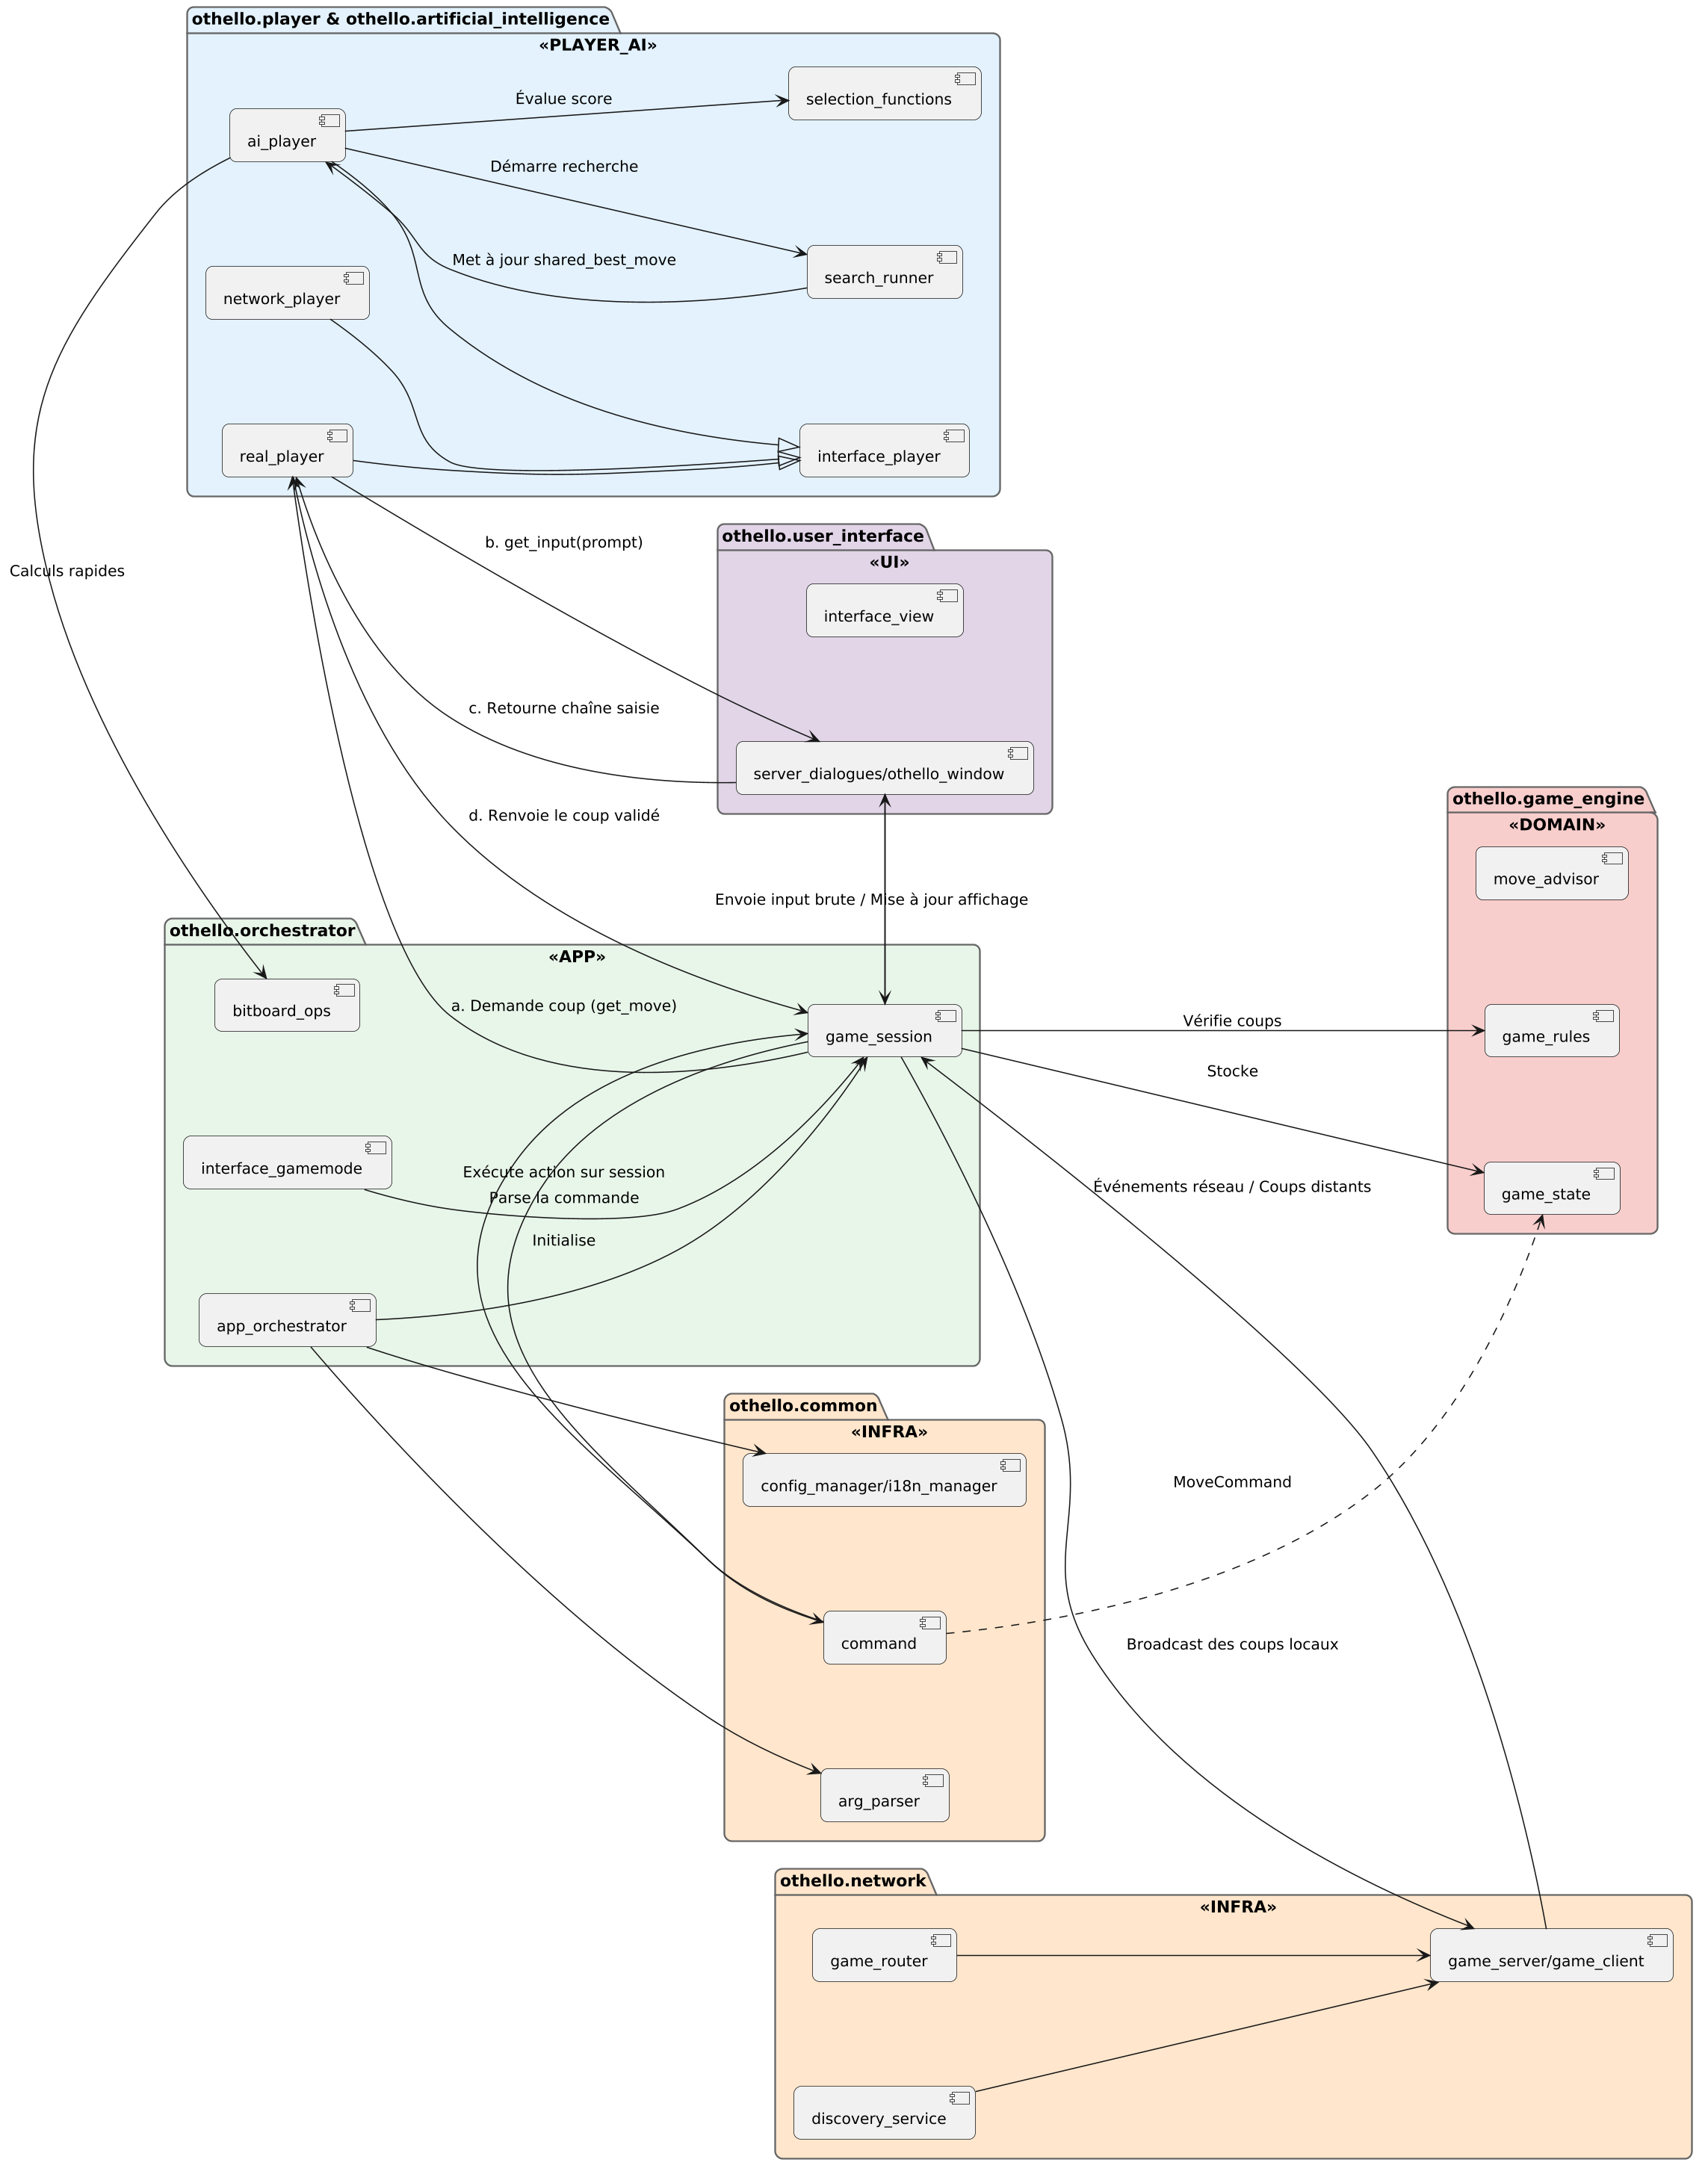
\includegraphics[width=0.9\textwidth]{images/uml.png}
    \caption{Dépendances principales du projet Othello}
    \label{fig:uml_arch}
\end{figure}

\section{Explication Approfondie : Intelligence artificielle}

\subsubsection{Intelligence Artificielle multi-stratégies (F31 à F37) \cite{OthelloSpecs2025}}
Le module d'Intelligence Artificielle (\texttt{ai\_player.py}) valide l'intégralité du cahier des charges sur les aspects algorithmiques :
\begin{itemize}
    \item \textbf{Gestion du temps (F31) \cite{OthelloSpecs2025}} : Le temps de réflexion est strictement borné et géré via un \texttt{threading.Event()} (\texttt{stop\_event}), permettant d'interrompre proprement la recherche de l'IA en cas de \textit{timeout}.
    \item \textbf{Algorithmes classiques (F32, F34, F35) \cite{OthelloSpecs2025}} : Le programme intègre l'algorithme Minimax optimisé via la variante \textbf{Negamax} avec élagage Alpha-Beta. De plus, un approfondissement itératif (\textit{Iterative Deepening}) a été implémenté via la méthode \texttt{it\_deepening}, permettant à l'algorithme d'affiner son choix jusqu'à l'interruption temporelle.
    \item \textbf{Heuristiques dynamiques (F33 \cite{OthelloSpecs2025})} : Trois fonctions d'évaluation distinctes sont disponibles dans \texttt{selection functions.py} : \texttt{positional\_eval}, \texttt{count\_stable\_discs}, et une fonction maîtresse \texttt{dynamic\_eval} qui bascule intelligemment de l'une à l'autre selon le pourcentage de remplissage du plateau.
    \item \textbf{MCTS et Machine Learning (F36, F37) \cite{OthelloSpecs2025}} : La Recherche Arborescente Monte-Carlo est implémentée avec une innovation majeure respectant l'exigence \textbf{F37} : la fonction de sélection classique UCB1 peut être remplacée par l'inférence d'un modèle de \textit{Deep Learning} (CNN via Keras) ou de \textit{Machine Learning} (Random Forest via joblib).
\end{itemize}

\subsubsection{Négamax et Élagage Alpha-Bêta}
Le moteur algorithmique historique est implémenté au sein de la classe \texttt{AIPlayer} par les méthodes \texttt{minimax()} et \texttt{negamax()}. L'algorithme repose sur Négamax, une variante élégante et concise de Minimax qui fusionne conceptuellement la minimisation et la maximisation. Le principe mathématique exploité veut que : maximiser son score équivaut à minimiser le score de l'adversaire. Ainsi, au lieu d'alterner code Min et code Max, on inverse systématiquement le signe du score retourné à chaque niveau de l'arbre.

Techniquement, la méthode récursive \texttt{negamax(state, current\_player, depth, alpha, beta)} scrute les arborescences. Si \texttt{depth == 0} ou si \texttt{GameRules.is\_terminal\_state()} est validé, l'évaluation heuristique est appelée sur la position. Sinon, la fonction itère sur les indices des coups générés par \texttt{get\_legal\_moves\_indices()}. Pour chaque coup, l'état de jeu est modifié via \texttt{apply\_move()}, puis l'algorithme s'y replonge en appelant récursivement \texttt{negamax(... , -beta, -alpha)}.

Pour accélérer de manière colossale cette recherche, l'élagage Alpha-Bêta y est intégré directement, s'appuyant sur les arguments :
\begin{itemize}
    \item \textbf{Alpha ($\alpha$)} : Le meilleur score formellement garanti pour le joueur courant.
    \item \textbf{Bêta ($\beta$)} : La limite maximale que l'adversaire est prêt à accepter sur cette branche.
\end{itemize}
Dès qu'un nœud révèle un score forçant $\alpha \geq \beta$, la boucle d'exploration est interrompue (\texttt{break}), élaguant de fait une branche entière des possibles.

\begin{figure}[H]
    \centering
    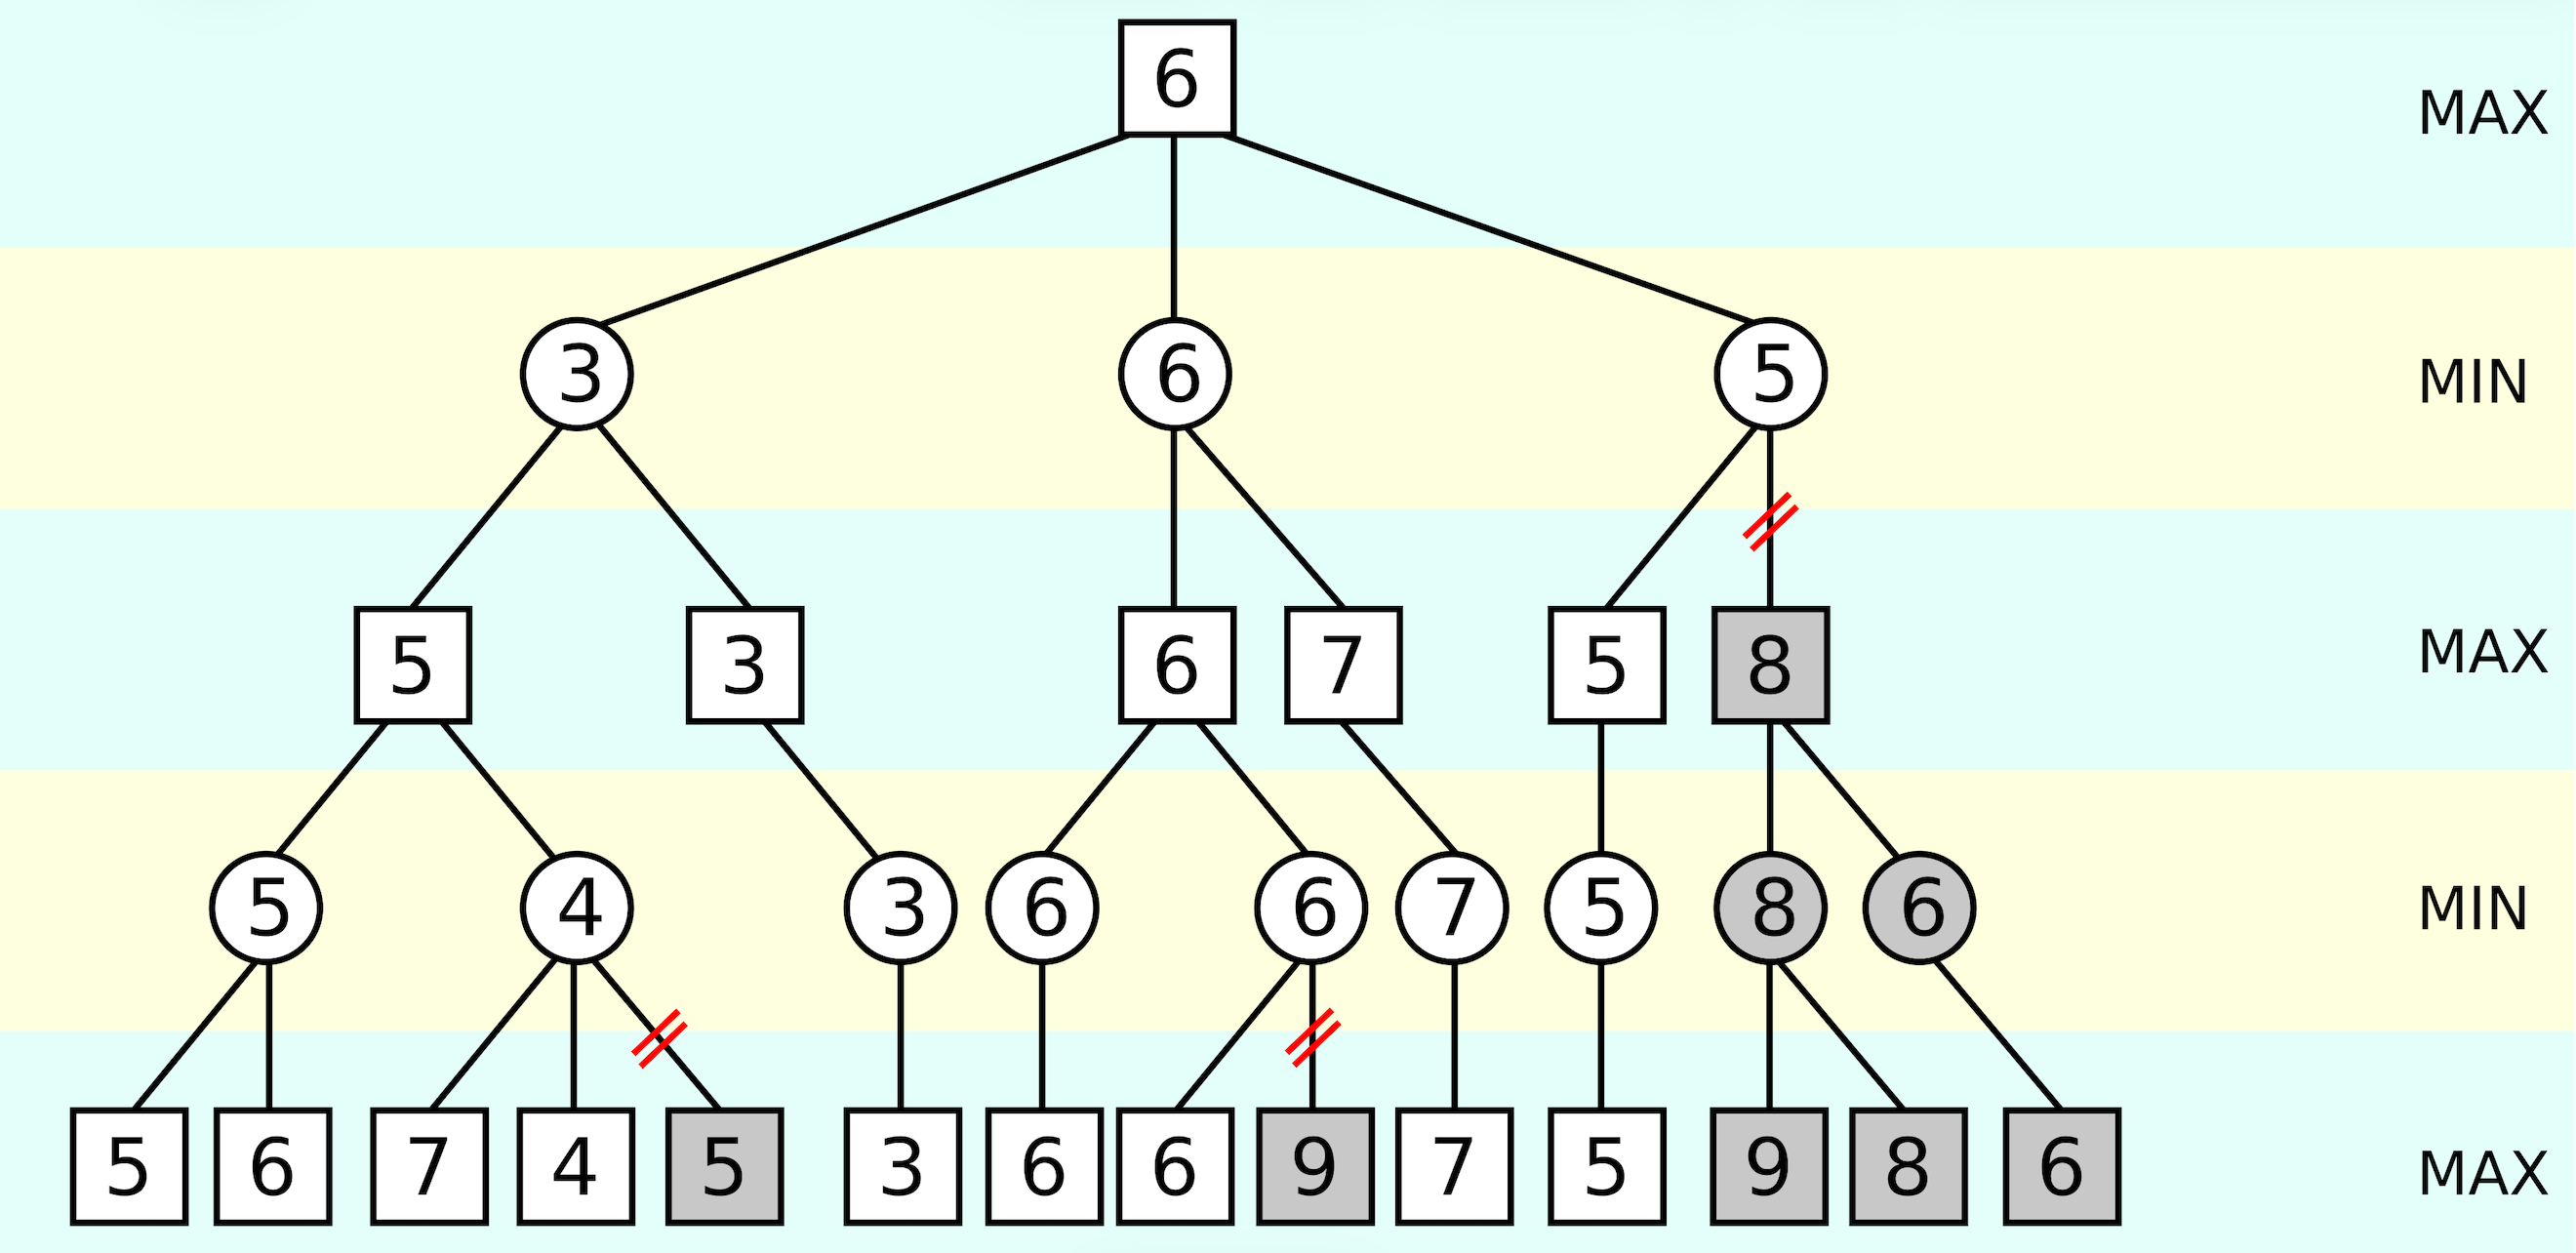
\includegraphics[width=0.4\textwidth]{images/minimax.png}
    \caption{wikipedia : Minimax avec élagage alpha-bêta}
\end{figure}

\subsubsection{Approfondissement Itératif (Iterative Deepening)}
Afin de maximiser l'utilisation du temps de réflexion octroyé sans risquer de rester bloqué au milieu d'une profonde exploration, la méthode \texttt{it\_deepening()} orchestre l'approche \textit{Iterative Deepening}.

Plutôt que de chercher aveuglément à une profondeur $N$ estimée, l'IA exécute sa recherche d'abord sur une profondeur 1, puis 2, de manière incrémentale. L'exécution est encapsulée dans une boucle \texttt{while current\_depth <= limit\_depth:} surveillée à chaque passe par l'évènement d'interruption réseau/utilisateur \texttt{self.stop\_event.is\_set()}. 
À la fin de chaque itération complète d'une profondeur déterminée, on sauvegarde formellement la réponse valide dans \texttt{self.shared\_best\_move} protégée par son verrou. Ainsi, si le \texttt{SearchRunner} coupe le flux au milieu d'une incursion d'arbre incomplète, le système repêchera de manière sécurisée la meilleure action finalisée à l'itération complète immédiatement précédente.

\subsubsection{Heuristiques d'Évaluation pour Minimax}
L'algorithme Négamax aboutit inévitablement sur un besoin d'évaluer le plateau. Le module dédié \texttt{selection\_functions.py} centralise nos heuristiques, agissant comme routeur via la méthode maîtresse \texttt{evaluate\_board()}. Selon le paramètre de configuration (\texttt{scoring\_func\_name}), elle va requérir l'appel d'une des trois fonctions d'estimations :
\begin{itemize}
    \item \textbf{Différence de pions (\texttt{default\_scoring})} : Ce calcul délègue au moteur (\texttt{GameRules.calculate\_score()}) la confrontation des \textit{bitboards} de la structure cible. Bien que rapide, la recherche de capture brute s'avère stratégiquement néfaste en début de partie et n'est redoutable qu'en toute fin d'arbre.
    \item \textbf{Évaluation positionnelle (\texttt{positional\_eval})} : Elle s'appuie sur le masque statique \texttt{BitboardOps.POSITIONAL\_HEURISTIC\_MASKS} pour attribuer des couches de poids aux différentes régions du plateau (coins extrêmes et bords intérieurs). Elle interroge bit à bit l'intersection logique (\(\&\)) entre le plateau du joueur \texttt{my\_bb} et les différents \texttt{mask} stratégiques.
    \item \textbf{Évaluation par stabilité pure (\texttt{stability\_eval})} : Appelant massivement la fonction interne \texttt{count\_stable\_discs}, elle définit l'acquisition absolue d'un pion (incapacité à être retourné dans le futur). Un disque est stable si ses quatre cordonnées (Horizontale, Verticale, Diagonales) sont rattachées perpétuellement au vide, aux bordures par les propres pions du joueur (\texttt{check\_side}), ou si les axes complets sont saturés sans cases libres.
\end{itemize}

\begin{figure}[H]
    \centering
    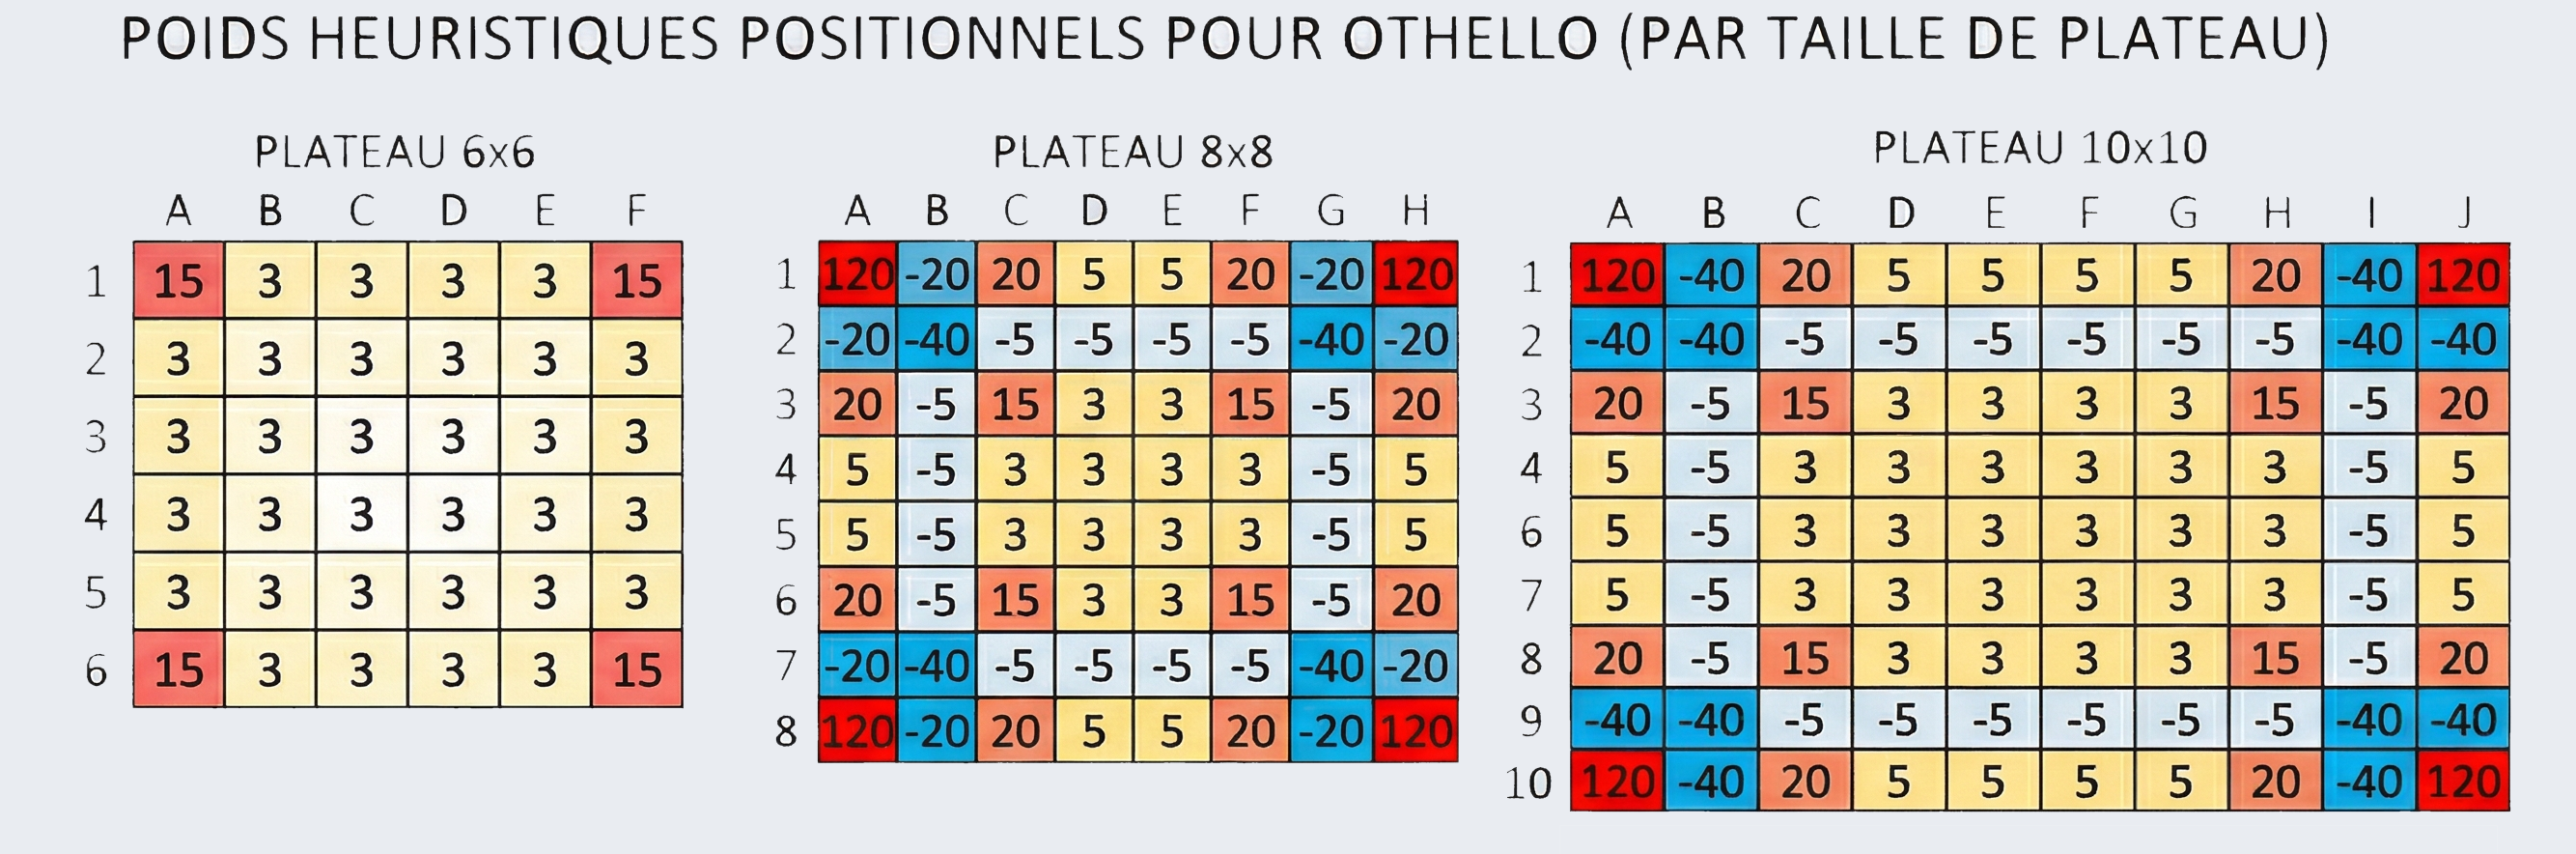
\includegraphics[width=0.7\textwidth]{images/positional_eval.png}
    \caption{Cartographie des pondérations des cases (Heuristique positionnelle).}
\end{figure}

Pour bénéficier constamment de la meilleure mesure, l'intelligence intègre sa propre heuristique adaptative, \texttt{dynamic\_eval}. Cette fonction lit le taux de remplissage structurel courant en calculant \texttt{progress = total\_pieces / total\_slots}. Suivant les pourcentages de ce \textit{ratio}, elle invoque l'évaluation pion-standard en dessous de 35\%, passe à l'analyse purement spatiale positionnelle en milieu de partie (jusqu'à 75\%), et enclenche le lourd calcul de stabilité absolue du plateau (\texttt{count\_stable\_discs}) pour les phases de conflit final.

\subsubsection{Monte Carlo Tree Search (MCTS) et UCT}
En marge du moteur classique, la méthode \texttt{mcts()} orchestre l'algorithme probabiliste asymétrique de l'Othello. L'architecture repose sur l'instanciation de données via la classe \texttt{MCTSNode}. Chaque nœud centralise son propre contexte abstrait : sa référence d'état immuable \texttt{state}, le score proportionnel \texttt{value}, le compte de visites empiriques \texttt{visits}, ainsi que ses options de branchements enfants (\texttt{children} ou \texttt{untried\_moves}).

Répétée par une boucle persistante \texttt{while True:} qui scrute l'interrupteur \texttt{self.stop\_event.is\_set()}, la recherche MCTS boucle ses quatre phases de vie itératives :
\begin{enumerate}
    \item \textbf{Sélection} : Depuis la racine \texttt{root}, on cascade récursivement en descendant l'arborescence via la \texttt{selection\_function} adéquate (\texttt{ucb1}). Cette phase évalue l'enfant idéal en itérant \texttt{max(node.children, key=...)} jusqu'à atteindre une feuille incomplète.
    \item \textbf{Expansion} : Tant qu'il subsiste des coups légaux (\texttt{node.untried\_moves}), l'algorithme sélectionne au hasard un index (\texttt{random.choice}), simule le couplage physique via la routine propre \texttt{GameRules.apply\_move()}, et instancie l'enfant résultant rajouté purement aux \texttt{node.children}.
    \item \textbf{Simulation (Rollout)} : Partant de cet environnement de travail naissant, le moteur s'embarque dans un combat sans règles ni algorithmiques : des pièces sont parachutées aléatoirement jusqu'à la saturation de la scène (quand \texttt{GameRules.is\_terminal\_state} déclare l'arrêt de la boucle). L'extracteur \texttt{determine\_winner} fixe instantanément un score final déterministe (1, -1 ou 0.5 en cas d'égalité matérielle).
    \item \textbf{Rétropropagation (Backpropagation)} : La récompense remonte récursivement les étages via la propriété parentale (\texttt{temp\_node.parent}), actualisant le total de simulation \texttt{visits} des parents traversés, et calibrant la prime relative incrémentée à la branche \texttt{value}.
\end{enumerate}
À son extinction coordonnée, on retient l'action enfant de \texttt{root} bénéficiant du ratio de visites majoritaire calculé par \texttt{max(root.children, key=lambda c: c.visits)}.

\begin{figure}[H]
    \centering
    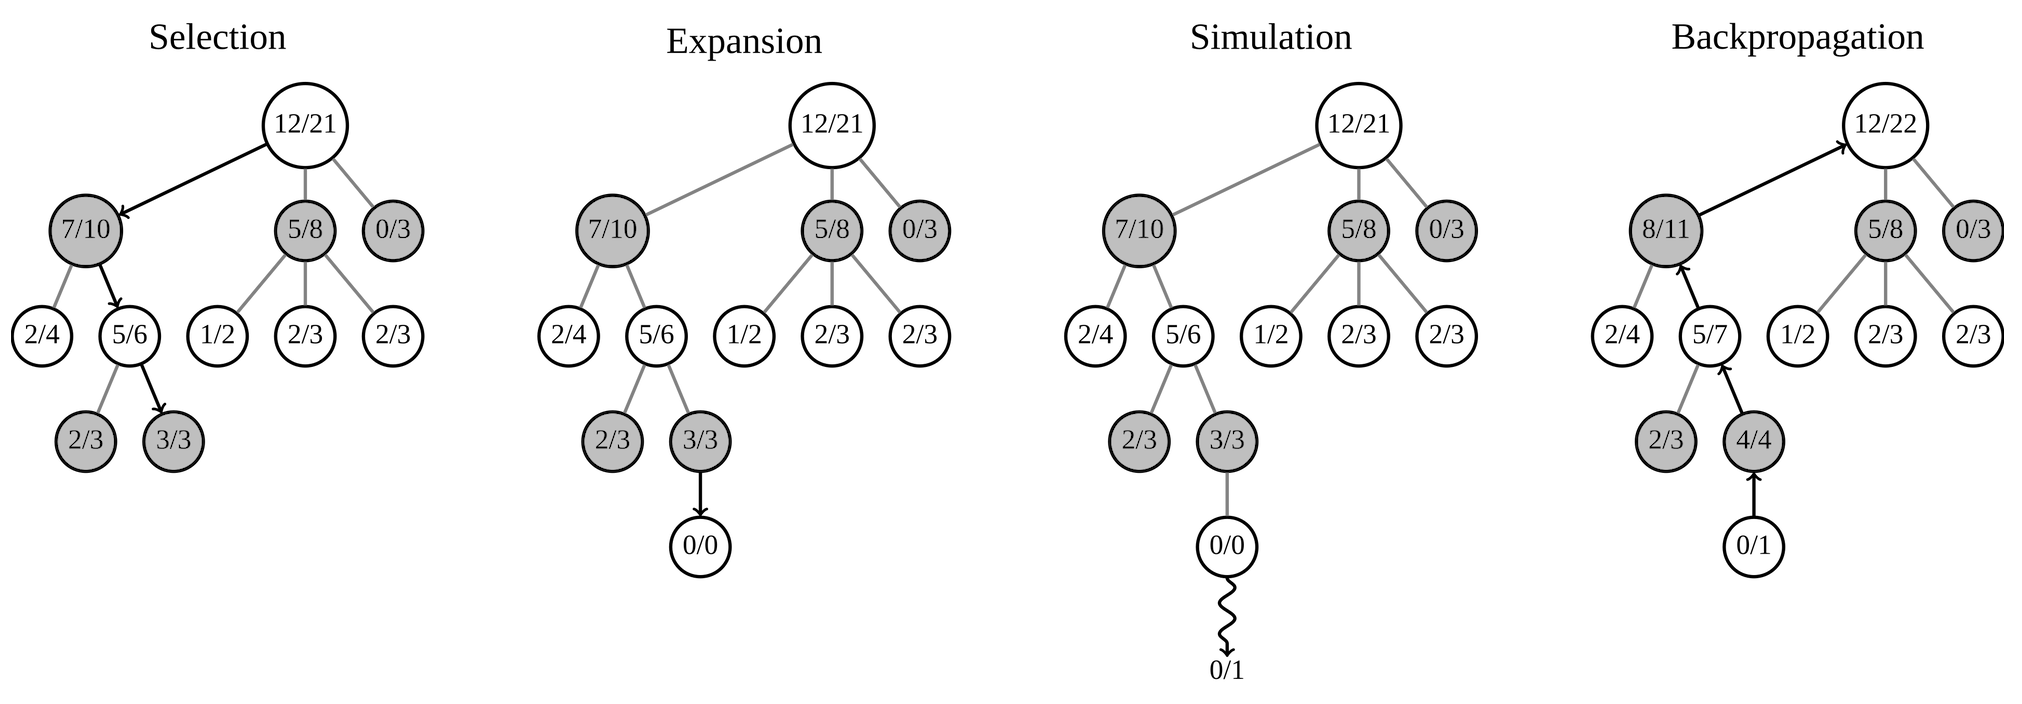
\includegraphics[width=\linewidth]{images/mcts.png}
    \caption{wikipedia : Recherche arborescente Monte-Carlo}
\end{figure}

\subsubsection{Intégration du Machine Learning dans la Sélection (Exigence F37)}

Conformément à l'exigence \textbf{F37} du cahier des charges \cite{OthelloSpecs2025}, le moteur dispose d'une fonction de sélection MCTS guidée par l'apprentissage automatique (Machine Learning). Cette approche supplante la formule mathématique d'exploration standard par une prédiction heuristique issue de l'expérience de jeu mémorisée par un algorithme d'apprentissage de type Random Forest ou Réseau Convolutif (CNN).

Dans la pratique, cette fonctionnalité dynamique est exposée à l'utilisateur via l'argument \texttt{--ai-mcts-selection} de l'interface en ligne de commande, acceptant les paramètres \texttt{UCT} (choisi par défaut) ou \texttt{ML}. Lorsque le mode \texttt{ML} est activé, l'orchestrateur charge au démarrage le modèle externe pré-entraîné.
Lors de l'étape de Sélection MCTS, le nœud itératif délègue sa décision à la méthode \texttt{ml\_dl\_selection}. Celle-ci convertit instantanément le \texttt{GameState} en matrice exploitable et l'injecte dans le modèle d'inférence, qui retourne un score continu de probabilité de victoire. L'algorithme se fie alors directement à cette intuition algorithmique globale pour isoler l'enfant le plus prometteur du nœud courant.

\textbf{L'équilibre de l'évaluation modulaire classique UCT}\\

Si l'utilisateur conserve le comportement par défaut (sans ML) dans son terminal d'exécution, afin de minimiser le regret décisionnel dans la passe initiale de Sélection, la méthode \texttt{ucb1} s'appuie sur la formule mathématique empirique suivante :

\[ UCT = \frac{v_i}{n_i} + c \sqrt{\frac{\ln(N)}{n_i}} \]

qui équilibre deux concepts fondamentaux :
\begin{itemize}
    \item \textbf{L'exploitation} : Capitalisée via l'attribut calculatoire brut d'espérance \(\texttt{node.value / node.visits}\), récompensant explicitement le fils actuellement le plus profitable du système parent.
    \item \textbf{L'exploration} : Poussant à l'exploration par l'enracinement mathématique \( \sqrt{\frac{\ln(\texttt{parent.visits})}{\texttt{node.visits}}} \) pondéré du scalaire d'équilibre \( \approx 1.414 \). Divisant par le \texttt{node.visits} local de l'enfant, l'expression croît exponentiellement lorsqu'une branche est délaissée, écrasant le calcul pour rendre ce fils prioritaire aux cycles limitrophes.
\end{itemize}

\subsection{Parallélisation du temps de réflexion IA (SearchRunner)}

Afin de gérer le temps de réflexion de l'intelligence artificielle de manière stricte, particulièrement lors de parties en mode Blitz, nous avons mis en œuvre l'exécution asynchrone et parallèle des algorithmes de recherche. La gestion de ce temps imparti est déléguée à une classe dédiée, \texttt{SearchRunner}. Son rôle est de lancer l'algorithme choisi (Négamax, \textit{Iterative Deepening} ou MCTS) dans un fil d'exécution isolé (\textit{background thread}). Ce choix architectural évite ainsi de figer l'interface utilisateur tout en garantissant un contrôle précis de la durée calculatoire.

\subsubsection*{Choix techniques et gestion des états partagés}

L'interface de communication entre le processus principal et le fil d'exécution de l'IA est bâtie autour de la classe \texttt{AIPlayer}. Lorsqu'une recherche de coup est lancée via la méthode \texttt{\_search\_task}, l'algorithme va consigner le dernier meilleur coup évalué dans la variable partagée \texttt{shared\_best\_move}. Pour prévenir toute corruption de données liée à des conditions de course (\textit{race conditions}), les lectures et écritures sur cette variable sont régies par un mécanisme de verrouillage asynchrone (\texttt{threading.Lock()} via l'attribut \texttt{move\_lock}).

L'orchestration temporelle est ensuite gérée conjointement par la fonction \texttt{run()} du \texttt{SearchRunner} :
\begin{enumerate}
    \item \textbf{Lancement et attente :} Le thread d'exploration est démarré et le thread principal attend passivement l'expiration du chronomètre alloué (via l'appel \texttt{thread.join(timeout)}).
    \item \textbf{Garantie d'un retour valide :} Si le délai est atteint mais qu'aucun coup légal n'a pu encore être identifié (la variable \texttt{shared\_best\_move} demeurant nulle), l'exécution continue son attente active par brefs verrous (\texttt{thread.join(0.01)}). Le jeu serait bloqué sans mouvement légal, il est donc impératif d'attendre l'évaluation d'au moins un coup de secours.
    \item \textbf{Arrêt coopératif :} Au moment où le temps est écoulé et qu'un coup valide est disposé en mémorisation, le système initie une procédure d'arrêt "propre". Il positionne l'évènement d'interruption coopératif (\texttt{stop\_event.set()}), interrogé depuis la boucle Python, pour notifier à l'algorithme l'interruption des itérations.
\end{enumerate}

\subsubsection*{Interruption des processus natifs bloqués (C API)}

Si, en dépit du signal coopératif \texttt{stop\_event}, le thread reste désespérément actif au-delà du court délai de grâce imparti (0,2 seconde), le système déclenche une exécution d'arrêt inconditionnelle (\textit{brutal kill}).

Cette démarche radicale est motivée par la nature native des dépendances du projet en \textit{Machine Learning}. Des appels sont déportés de l'interprète Python vers ces modules externes compilés purement en C. Sur ce point, les conventions du langage Python s'arrêtent : une instruction classique pour lever une exception ignorera les procédures en cours de ces couches internes.

Pour forcer cette transition de manière infaillible, le module originel \texttt{ctypes} de l'API C de Python expose la primitive la plus critique et efficace du langage : \texttt{PyThreadState\_SetAsyncExc}. Cet appel de très bas niveau superpose l'erreur vitale dans les registres du fil parent. L'état virtuel injectera de lui-même l'exception \texttt{SearchTimeout} sans attente, neutralisant alors les opérations au sein des nœuds en C, confisquant et libérant subitement cette lourde occupation mémoire.

Dans le cadre de l'élaboration d'une Intelligence Artificielle pour notre moteur d'Othello, nous avons fait le choix d'explorer et de comparer deux approches distinctes : un modèle d'apprentissage classique (Random Forest) et un réseau de neurones convolutif profond (CNN). L'objectif est de pouvoir évaluer la pertinence d'un coup de manière instantanée, en complément ou en remplacement de l'algorithme Minimax classique.

\subsection{Constitution et ingénierie des données (Dataset)}

La création d'un modèle décisionnel performant requiert un volume massif de données de qualité. Notre démarche de constitution du jeu de données s'est déroulée en deux phases distinctes : l'exploitation d'une base de données existante, et la génération d'environnements de jeu de différentes tailles.

Au terme de ce processus, notre jeu de données final regroupe un million de positions (états de plateau uniques) extraites de 200 000 parties complètes d'Othello. Afin d'entraîner un modèle robuste et performant sur tous les formats possibles, ce \textit{dataset} arbore une répartition structurelle équilibrée : 15\% de grilles 6x6, 50\% de grilles 8x8 (combinant les historiques et les synthétiques), 15\% de grilles 10x10, et enfin 20\% de grilles 12x12.

\subsubsection{Traduction et formatage de données historiques}
Pour amorcer l'apprentissage, nous nous sommes appuyés sur un jeu de données public issu de la plateforme Kaggle \cite{KaggleOthello}, regroupant des milliers de parties d'Othello au format standard (8x8). Cependant, ces données brutes n'étaient pas exploitables en l'état : les parties y étaient retranscrites sous forme de chaînes de caractères de notation algébrique (ex: \verb|"e6f4c3..."|).

Afin d'en extraire des matrices d'apprentissage, nous avons développé le module \texttt{ModelTrainer}. La méthode \texttt{play\_game\_from\_moves} agit comme un parseur syntaxique : elle lit la chaîne de caractères, traduit les coordonnées (\verb|ord(col_str) - ord("a")|) et rejoue virtuellement la partie entière sur notre moteur de \textit{Bitboards}. À intervalles réguliers (tant que le plateau n'est pas rempli à plus de 78\%), l'état de la partie est capturé et sauvegardé.

Ce seuil d'arrêt à 78\% est un choix délibéré d'ingénierie des données. En effet, la fin de partie à Othello se caractérise par une réduction drastique du facteur de branchement, rendant les derniers coups purement déterministes et facilement résolubles de manière exacte par un simple algorithme Minimax. Exclure ces états finaux empêche les modèles d'apprentissage de gaspiller leur capacité de mémorisation sur des séquences forcées ou des victoires triviales, les forçant ainsi à développer une véritable "intuition" heuristique sur les phases complexes d'ouverture et de milieu de partie.

Selon le modèle cible, l'état est ensuite exporté soit sous forme de vecteur plat de 144 variables (correspondant aux cases du plateau maximal 12x12) pour le \textit{Random Forest} (\textit{flat}), soit sous forme de grille bidimensionnelle pour le CNN (\textit{2d}).

\subsubsection{Génération synthétique et augmentation des données}
Le jeu de données Kaggle présentait une limitation majeure vis-à-vis de notre cahier des charges : il se cantonnait exclusivement au format 8x8. Or, notre Intelligence Artificielle devait être agnostique et capable de jouer sur des plateaux allant de 6x6 à 12x12.

Pour pallier ce manque, le \texttt{ModelTrainer} a été conçu pour générer ses propres données de manière autonome. Nous avons orchestré des affrontements automatisés entre des agents \textit{Minimax} (utilisant l'élagage Alpha-Beta avec une profondeur de 4) sur des plateaux de tailles 6x6, 10x10 et 12x12. Cette approche, appelée "augmentation de données" (\textit{Data Augmentation}), a permis de :
\begin{itemize}
    \item \textbf{Diversifier la dimension spatiale :} Fournir au réseau convolutif des exemples de bords et de coins à des distances variables, justifiant l'utilisation ultérieure du \texttt{GlobalMax Pooling2D}.
    \item \textbf{Élever le niveau stratégique :} L'utilisation du \textit{Minimax} garantit que les situations de plateau générées sont tactiquement réalistes et complexes, évitant ainsi d'entraîner le modèle sur des séquences de coups aléatoires ou absurdes.
\end{itemize}

\subsection{Préparation et purification des données}
La qualité d'un modèle prédictif dépendant intrinsèquement de ses données d'entraînement, une phase de traitement s'est imposée. Lors de nos premiers essais, le modèle utilisait une perte \verb|binary_crossentropy| où les victoires des Noirs valaient 1 et celles des Blancs -1 (converties en 0 par la suite). Le modèle confondait alors systématiquement une partie nulle et une victoire des Blancs.

Pour corriger ce biais bloquant l'apprentissage, nous avons procédé à la suppression des parties donnant un résultat nul, car l'absence de vainqueur net est ininterprétable pour une classification binaire au sein du CNN.

\subsection{Modèle de Machine Learning : Random Forest}
\subsubsection{Architecture et Hyperparamètres}
Notre première approche repose sur un classifieur de type Random Forest. Afin de garantir un modèle léger (inférieur à 200 Mo) et rapide d'exécution sur processeur (CPU) pour l'inférence en temps réel, nous avons bridé l'algorithme. Les paramètres \verb|max_leaf_nodes=25000| et \verb|n_estimators=40| ont parfaitement joué leur rôle de régulateurs.

\subsection{Modèle de Deep Learning : Réseau de Neurones Convolutif (CNN)}
\subsubsection{Choix architecturaux}
Pour exploiter la nature purement spatiale du jeu d'Othello, une architecture convolutive a été développée. Une modification majeure a été le remplacement de la traditionnelle couche Flatten() par une couche GlobalMaxPooling2D(). En jeu réel, cela permet à l'IA de recevoir une matrice 6x6 ou 12x12 et de l'analyser directement sans aucun padding. L'atout majeur technique du \verb|GlobalMaxPooling2D()| réside dans le fait qu'il va regarder chaque carte de caractéristiques (chaque filtre de taille N x N) et ne conserver que la valeur maximale, indépendamment de sa position spatiale.

Ce mécanisme transforme une information du type "Il y a un motif de victoire aux coordonnées (X, Y)" en "Il y a un motif de victoire QUELQUE PART sur le plateau". Peu importe la taille du plateau, la couche de Pooling sortira toujours un vecteur fixe de taille 512 (car il y a 512 filtres à la couche précédente). C'est ce qui rend notre IA totalement adaptable à la taille de la grille.

Puisque le \verb|GlobalMaxPooling2D| fait perdre l'information des coordonnées exactes, l'architecture a été renforcée (les convolutions passent de 128 à 256, puis 512 filtres). L'objectif est de forcer les couches de convolution à détecter des "motifs" très complexes avant que l'information spatiale ne soit compressée par le Pooling. Enfin, la prédiction finale est assurée par une couche \verb|Dense(1, activation="sigmoid")| offrant une seule sortie écrasée entre 0 et 1. Si le score est proche de 1, les Noirs gagnent ; s'il est proche de 0, les Blancs gagnent.

\subsubsection{Optimisation et contrôle de l'apprentissage}
Pour prévenir la mémorisation excessive du dataset, nous avons fait l'utilisation d'un \verb|Dropout(0.5)| massif sur les couches \verb|Dense| finales. La stabilisation du gradient a été assurée par l'ajout de couches \verb|BatchNormalization()|, ce qui recentre mathématiquement les activations après chaque convolution et évite l'explosion ou la disparition des valeurs, accélérant grandement la convergence sur GPU.

Le contrôle de l'entraînement a été automatisé via des callbacks de l'API Keras. D'une part, l'outil \textbf{EarlyStopping} est utilisé au lieu de forcer les 40 époques bêtement : le script surveille la perte sur le jeu de validation (\verb|val_loss|). S'il voit que le modèle commence à apprendre le jeu par cœur au détriment de l'inconnu, il coupe l'entraînement et restaure automatiquement la meilleure version du modèle. D'autre part, \textbf{ReduceLROnPlateau} affine le gradient quand l'apprentissage ralentit, en divisant la taille de ses "pas d'apprentissage" (learning rate) par 2.

Sur le plan matériel, l'utilisation de types \verb|float32| et l'augmentation de la taille des batchs ont permis de saturer intelligemment la VRAM de la carte graphique et d'accélérer l'entraînement via les bibliothèques XLA/CUDA de TensorFlow.

\section{Explication Approfondie : Architecture Réseau Multi-clients}

L'ajout de fonctionnalités multijoueurs à notre moteur d'Othello a nécessité la conception d'une architecture réseau robuste, capable de gérer des requêtes concurrentes, des déconnexions inopinées et la synchronisation des états de jeu entre plusieurs machines. Contrairement à une simple implémentation de sockets bloquants, nous avons opté pour une architecture client-serveur multithreadée, découpée en services spécialisés.

\section{Explication Approfondie : Architecture Réseau Multi-clients}

L'ajout de fonctionnalités multijoueurs à notre moteur d'Othello a nécessité la conception d'une architecture réseau capable de gérer plusieurs requêtes simultanément, des déconnexions imprévues et la synchronisation des plateaux de jeu entre les machines. Nous avons opté pour une architecture client-serveur basée sur des processus légers (\textit{threads}), découpée en plusieurs modules spécialisés.

\begin{figure}[H]
    \centering
    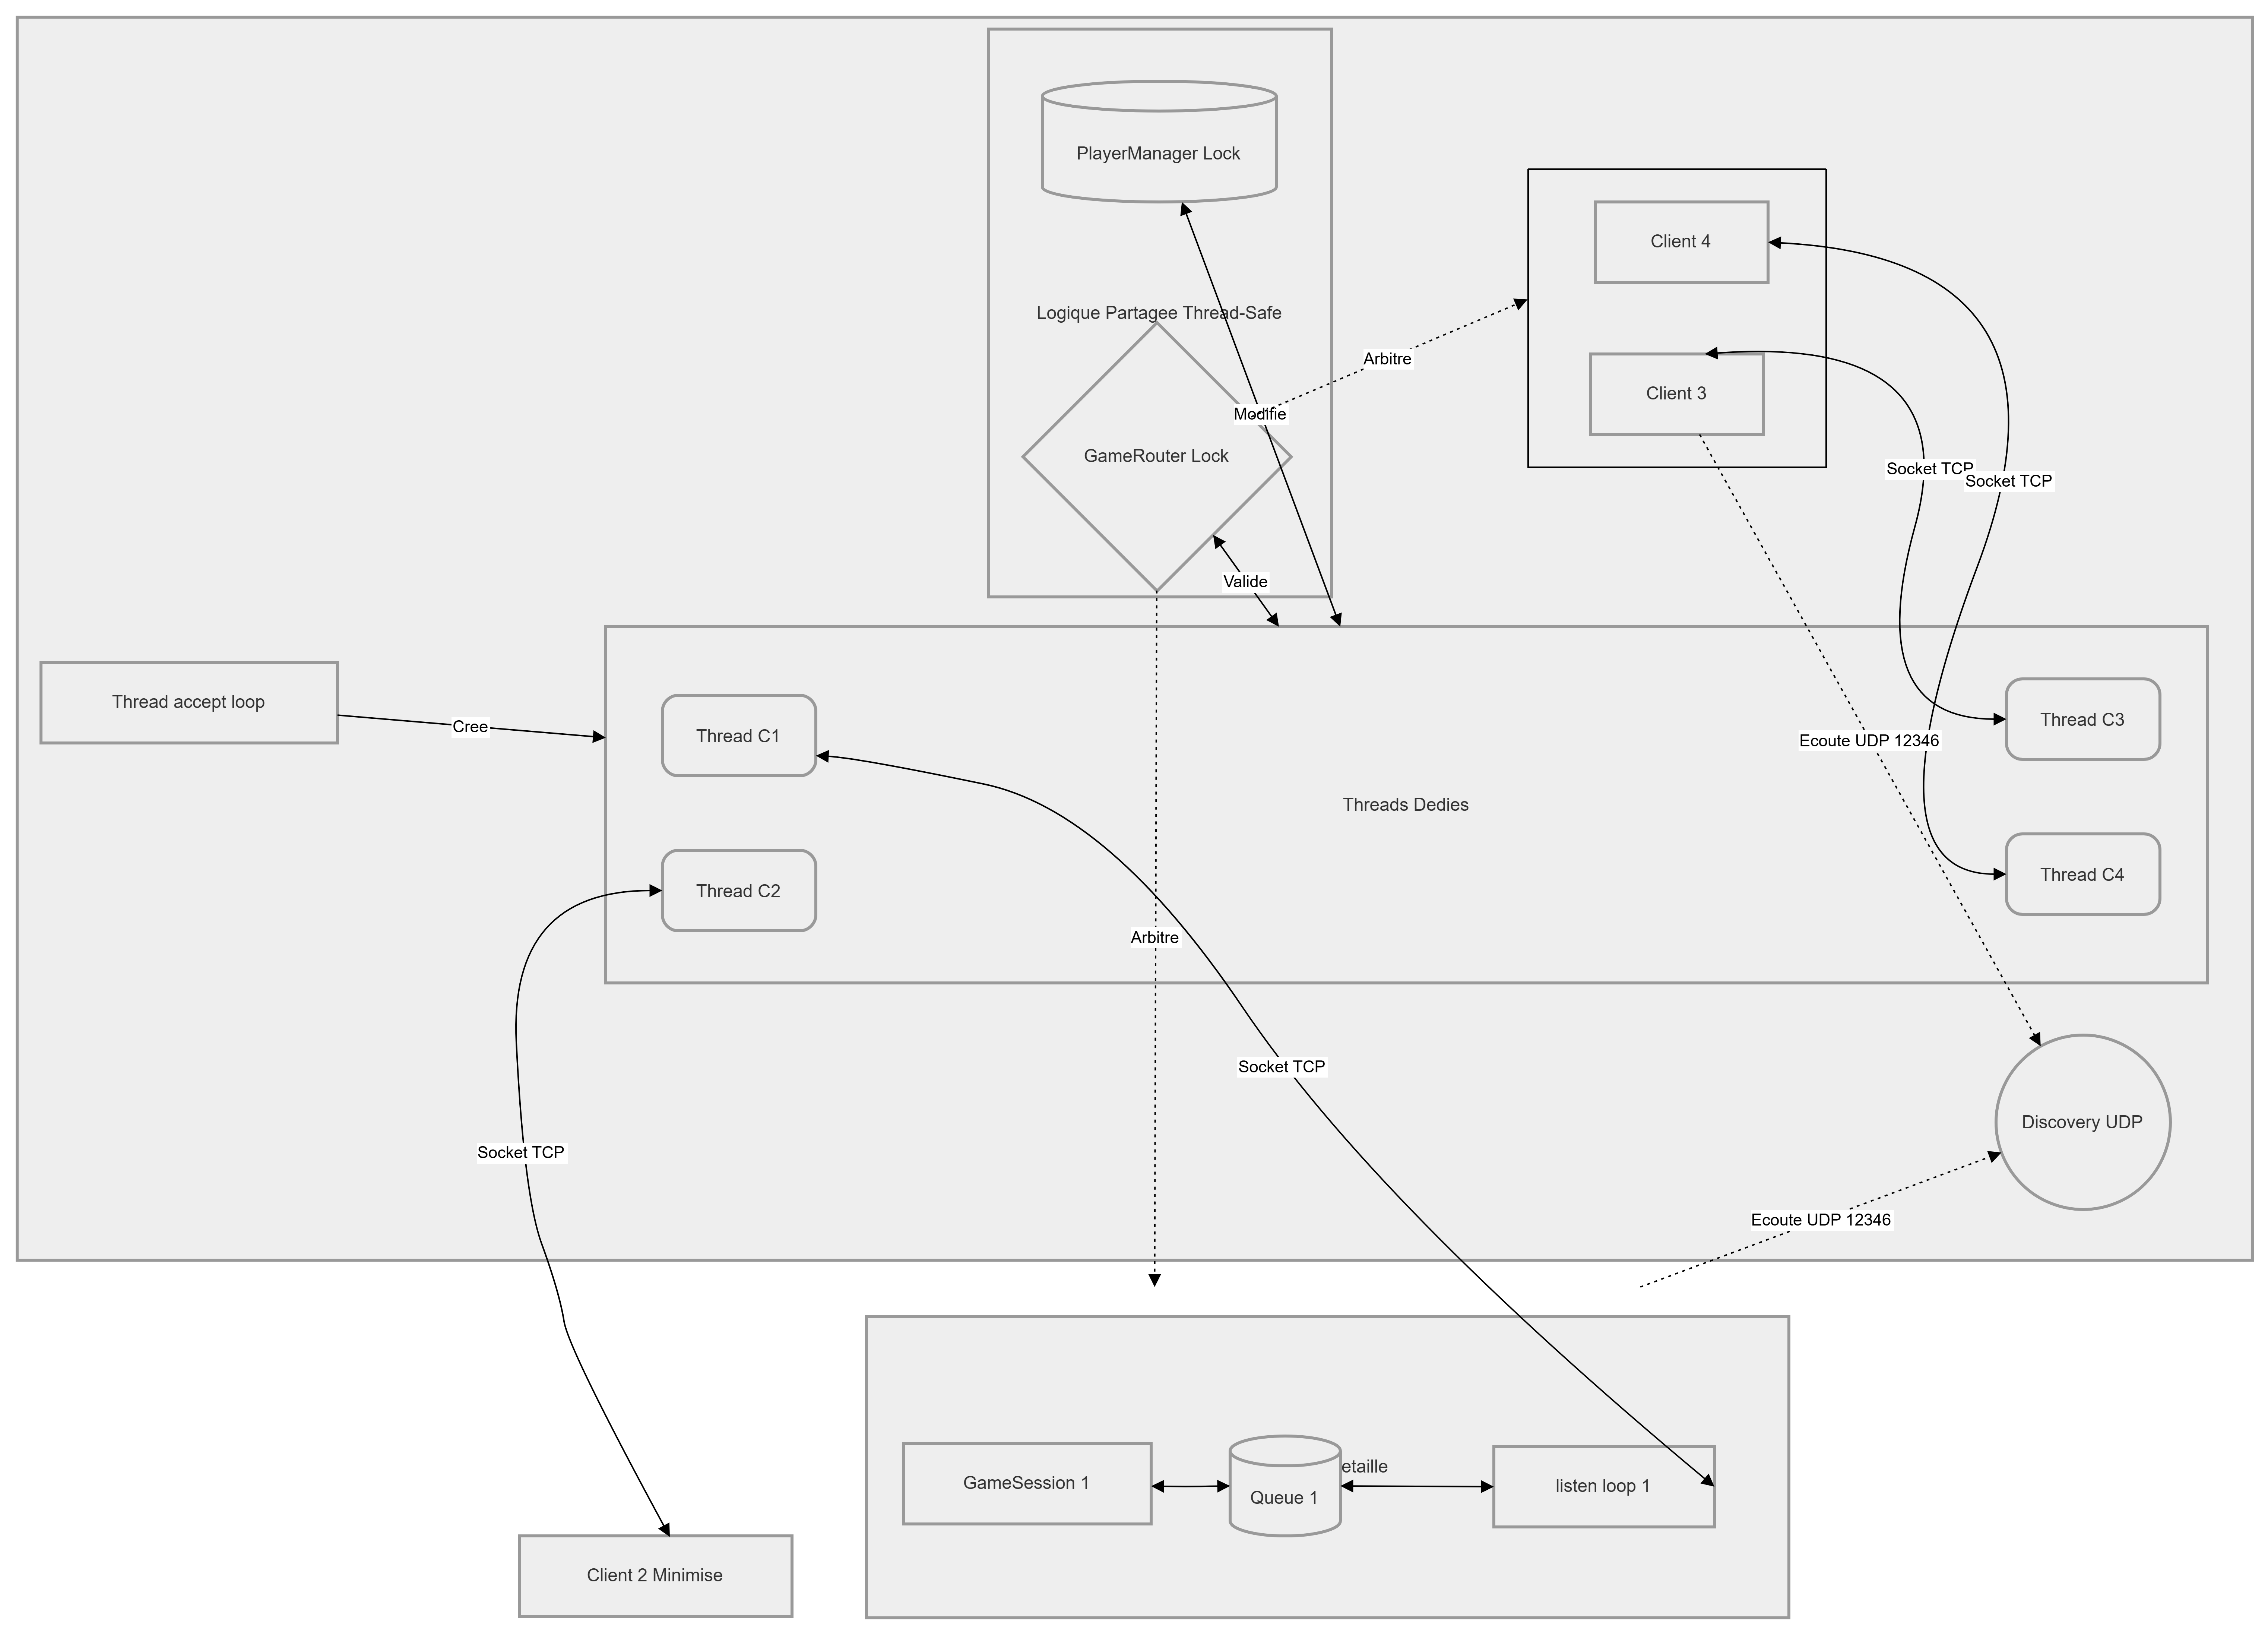
\includegraphics[width=\textwidth]{images/multithreadserver.png}
    \caption{Architecture réseau globale : Le serveur centralise les requêtes via des threads dédiés, gère la découverte UDP et arbitre les parties.}
    \label{fig:network_arch_global}
\end{figure}

\subsection{L'architecture côté Serveur : Structure détaillée des modules}

Le cahier des charges exigeait qu'un serveur puisse gérer plusieurs clients simultanément (exigence \textbf{F39}). Pour y répondre, notre serveur a été structuré autour de trois classes principales, toutes sécurisées par des verrous d'exclusion mutuelle (\texttt{threading.Lock()}) pour éviter les conflits d'accès aux données.

\textbf{1. La classe \texttt{GameServer} et la boucle d'acceptation}\\
Il s'agit du module principal du serveur, responsable des connexions TCP entrantes (sur le port 12345 par défaut). Plutôt que de bloquer l'exécution du programme à chaque connexion, cette classe s'appuie sur la méthode \texttt{\_accept\_loop} (illustrée par la Figure \ref{fig:accept_loop_server}). 
Cette boucle écoute le port TCP en continu. Dès qu'un client se connecte, la boucle ne traite pas les données elle-même : elle crée un fil d'exécution (\textit{thread}) démon \texttt{\_handle\_client} dédié spécifiquement à ce joueur, puis retourne immédiatement écouter le port. Ce mécanisme permet d'accepter de nombreuses connexions à la suite sans interruption.

\begin{figure}[H]
    \centering
    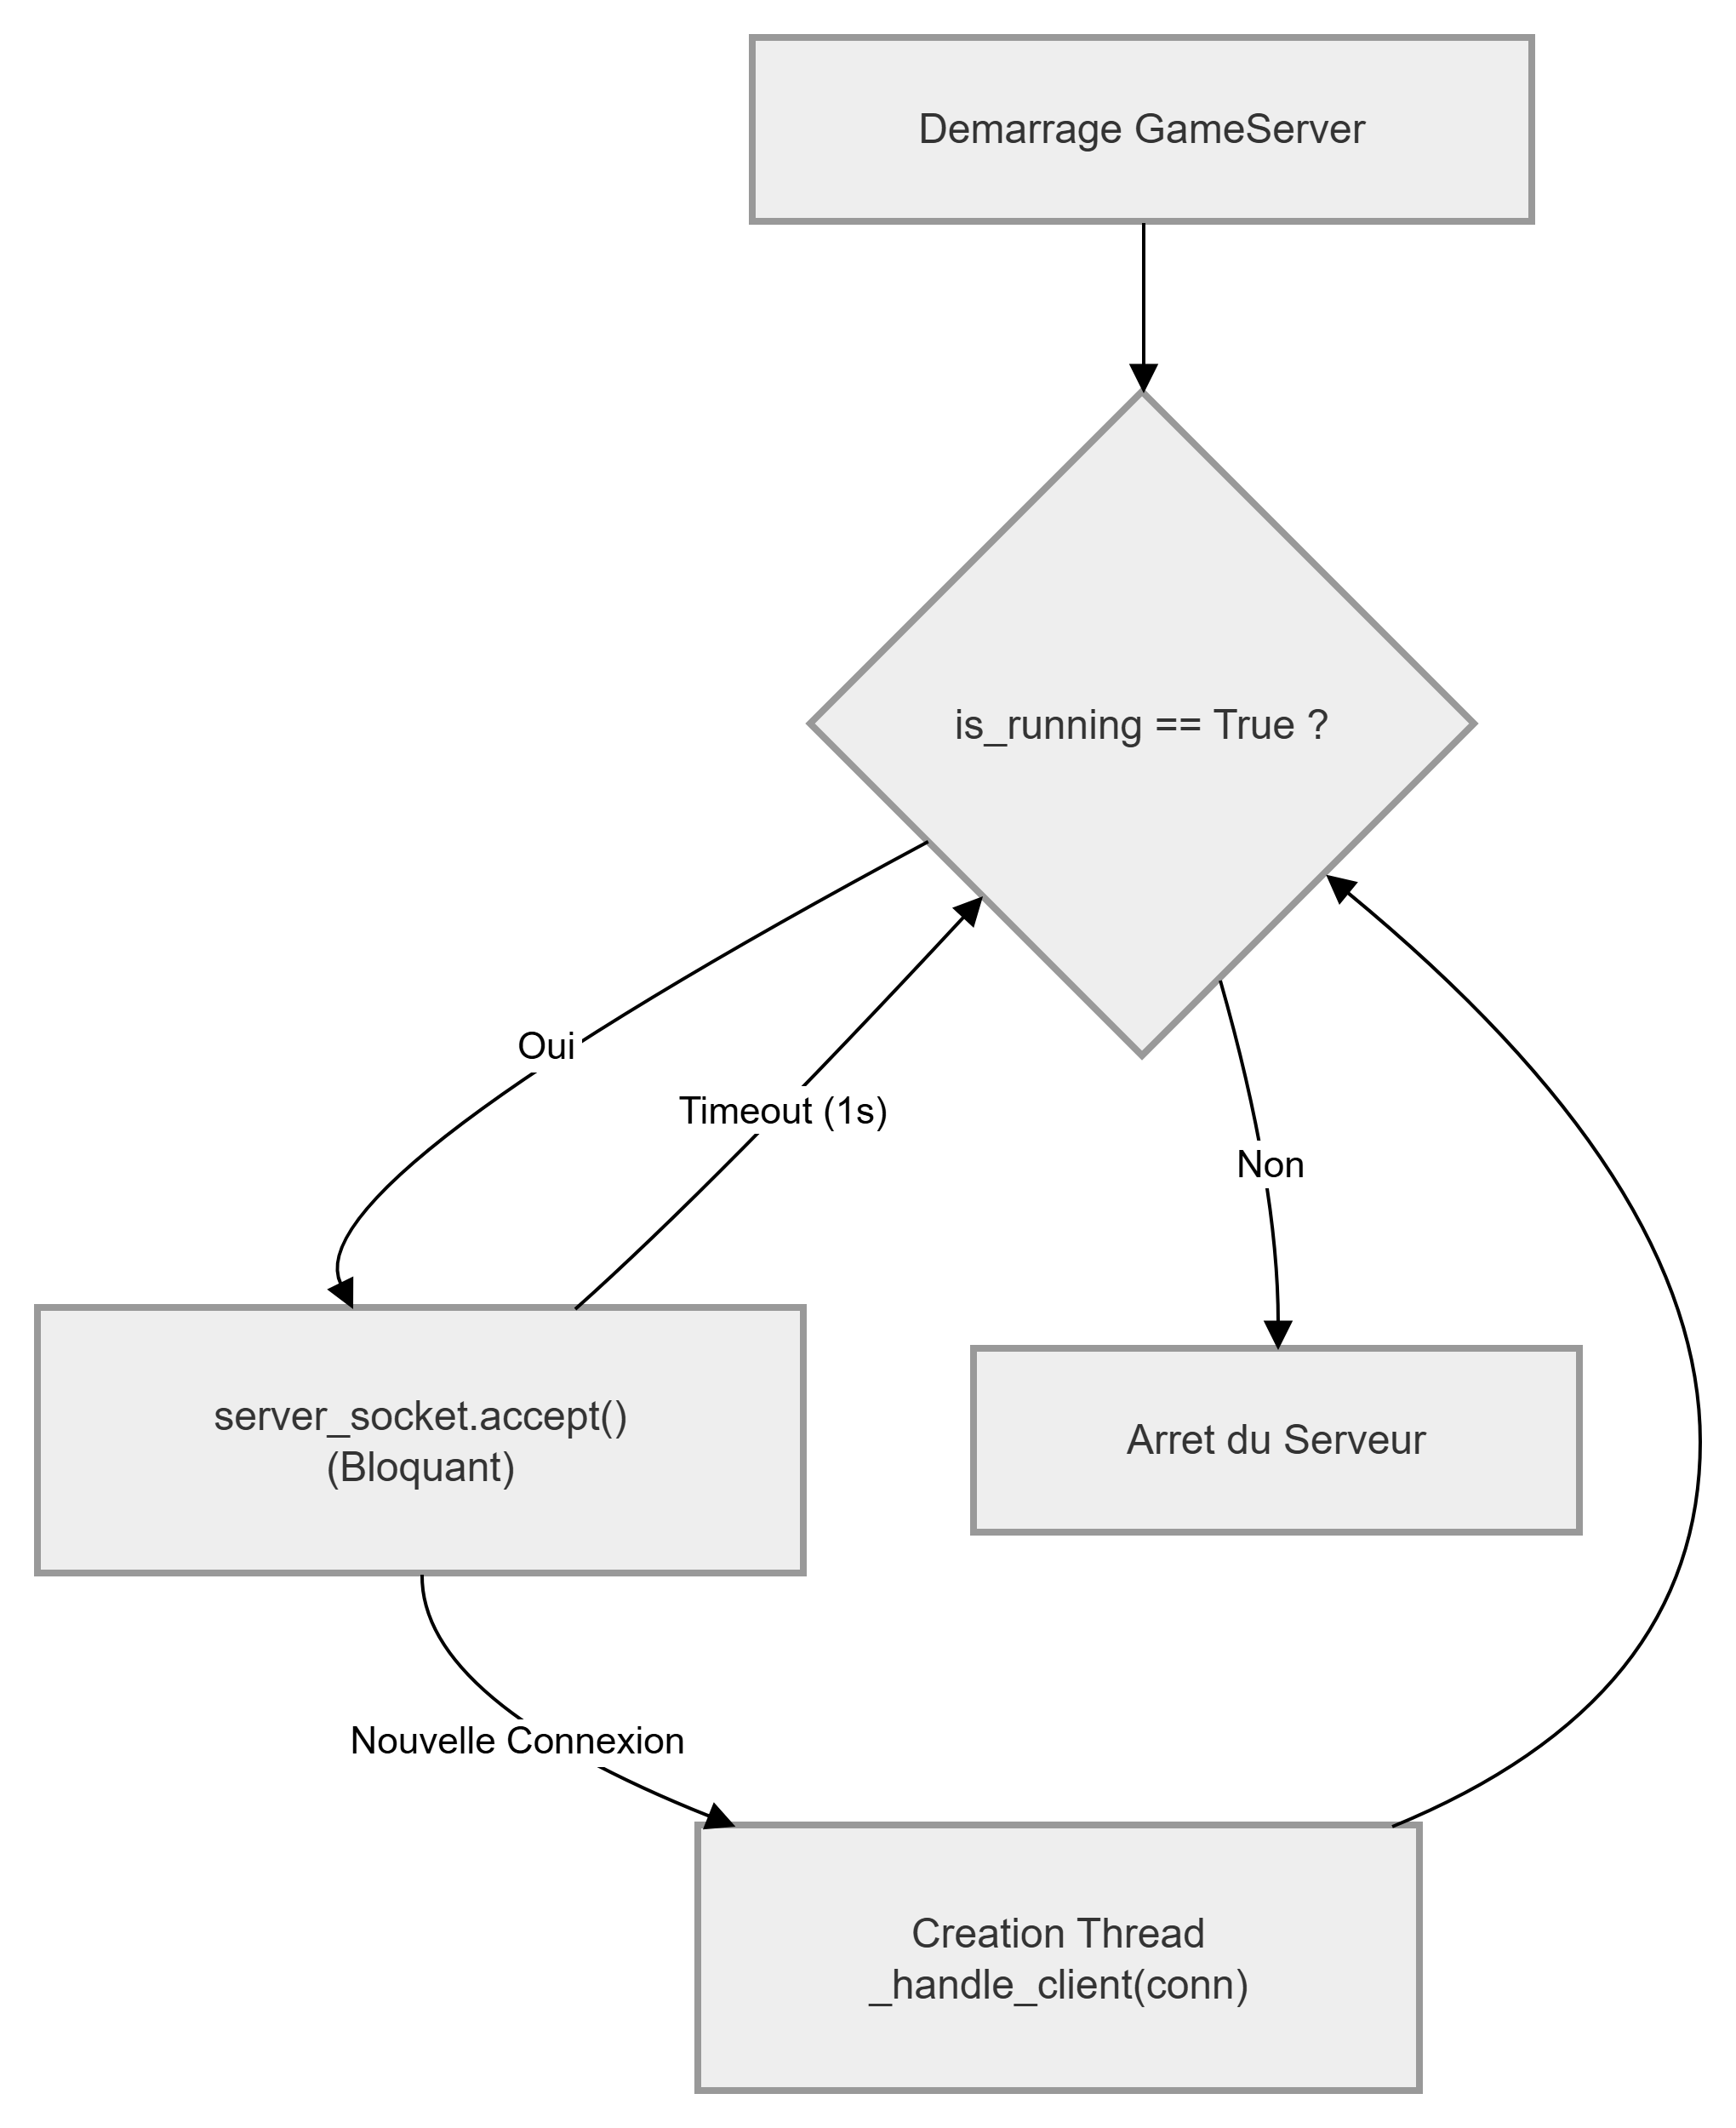
\includegraphics[width=0.4\textwidth]{images/accept_loop_server.png}
    \caption{Mécanique de la boucle d'acceptation (\texttt{\_accept\_loop}) dans le GameServer.}
    \label{fig:accept_loop_server}
\end{figure}

\textbf{2. La classe \texttt{PlayerManager} (Gestion des profils)}\\
Ce module agit comme la base de données interne du serveur. Il lie chaque connexion technique à un profil de joueur logique. Il attribue un identifiant unique (ex: \texttt{Player\_1}), maintient le tableau des scores (\texttt{scoreboard}), et suit l'état des joueurs (\texttt{idle}, \texttt{away}, \texttt{waitgame}, \texttt{ingame}) pour satisfaire l'exigence \textbf{F40}.
Une de ses fonctionnalités clés est le traitement des changements de pseudonyme. Lorsqu'un client utilise la commande \texttt{NAME}, le \texttt{PlayerManager} vérifie la disponibilité du pseudonyme, puis fusionne les statistiques (victoires/défaites) de l'ancien identifiant avec le nouveau de manière transparente (voir Figure \ref{fig:sequence_name}).

\begin{figure}[H]
    \centering
    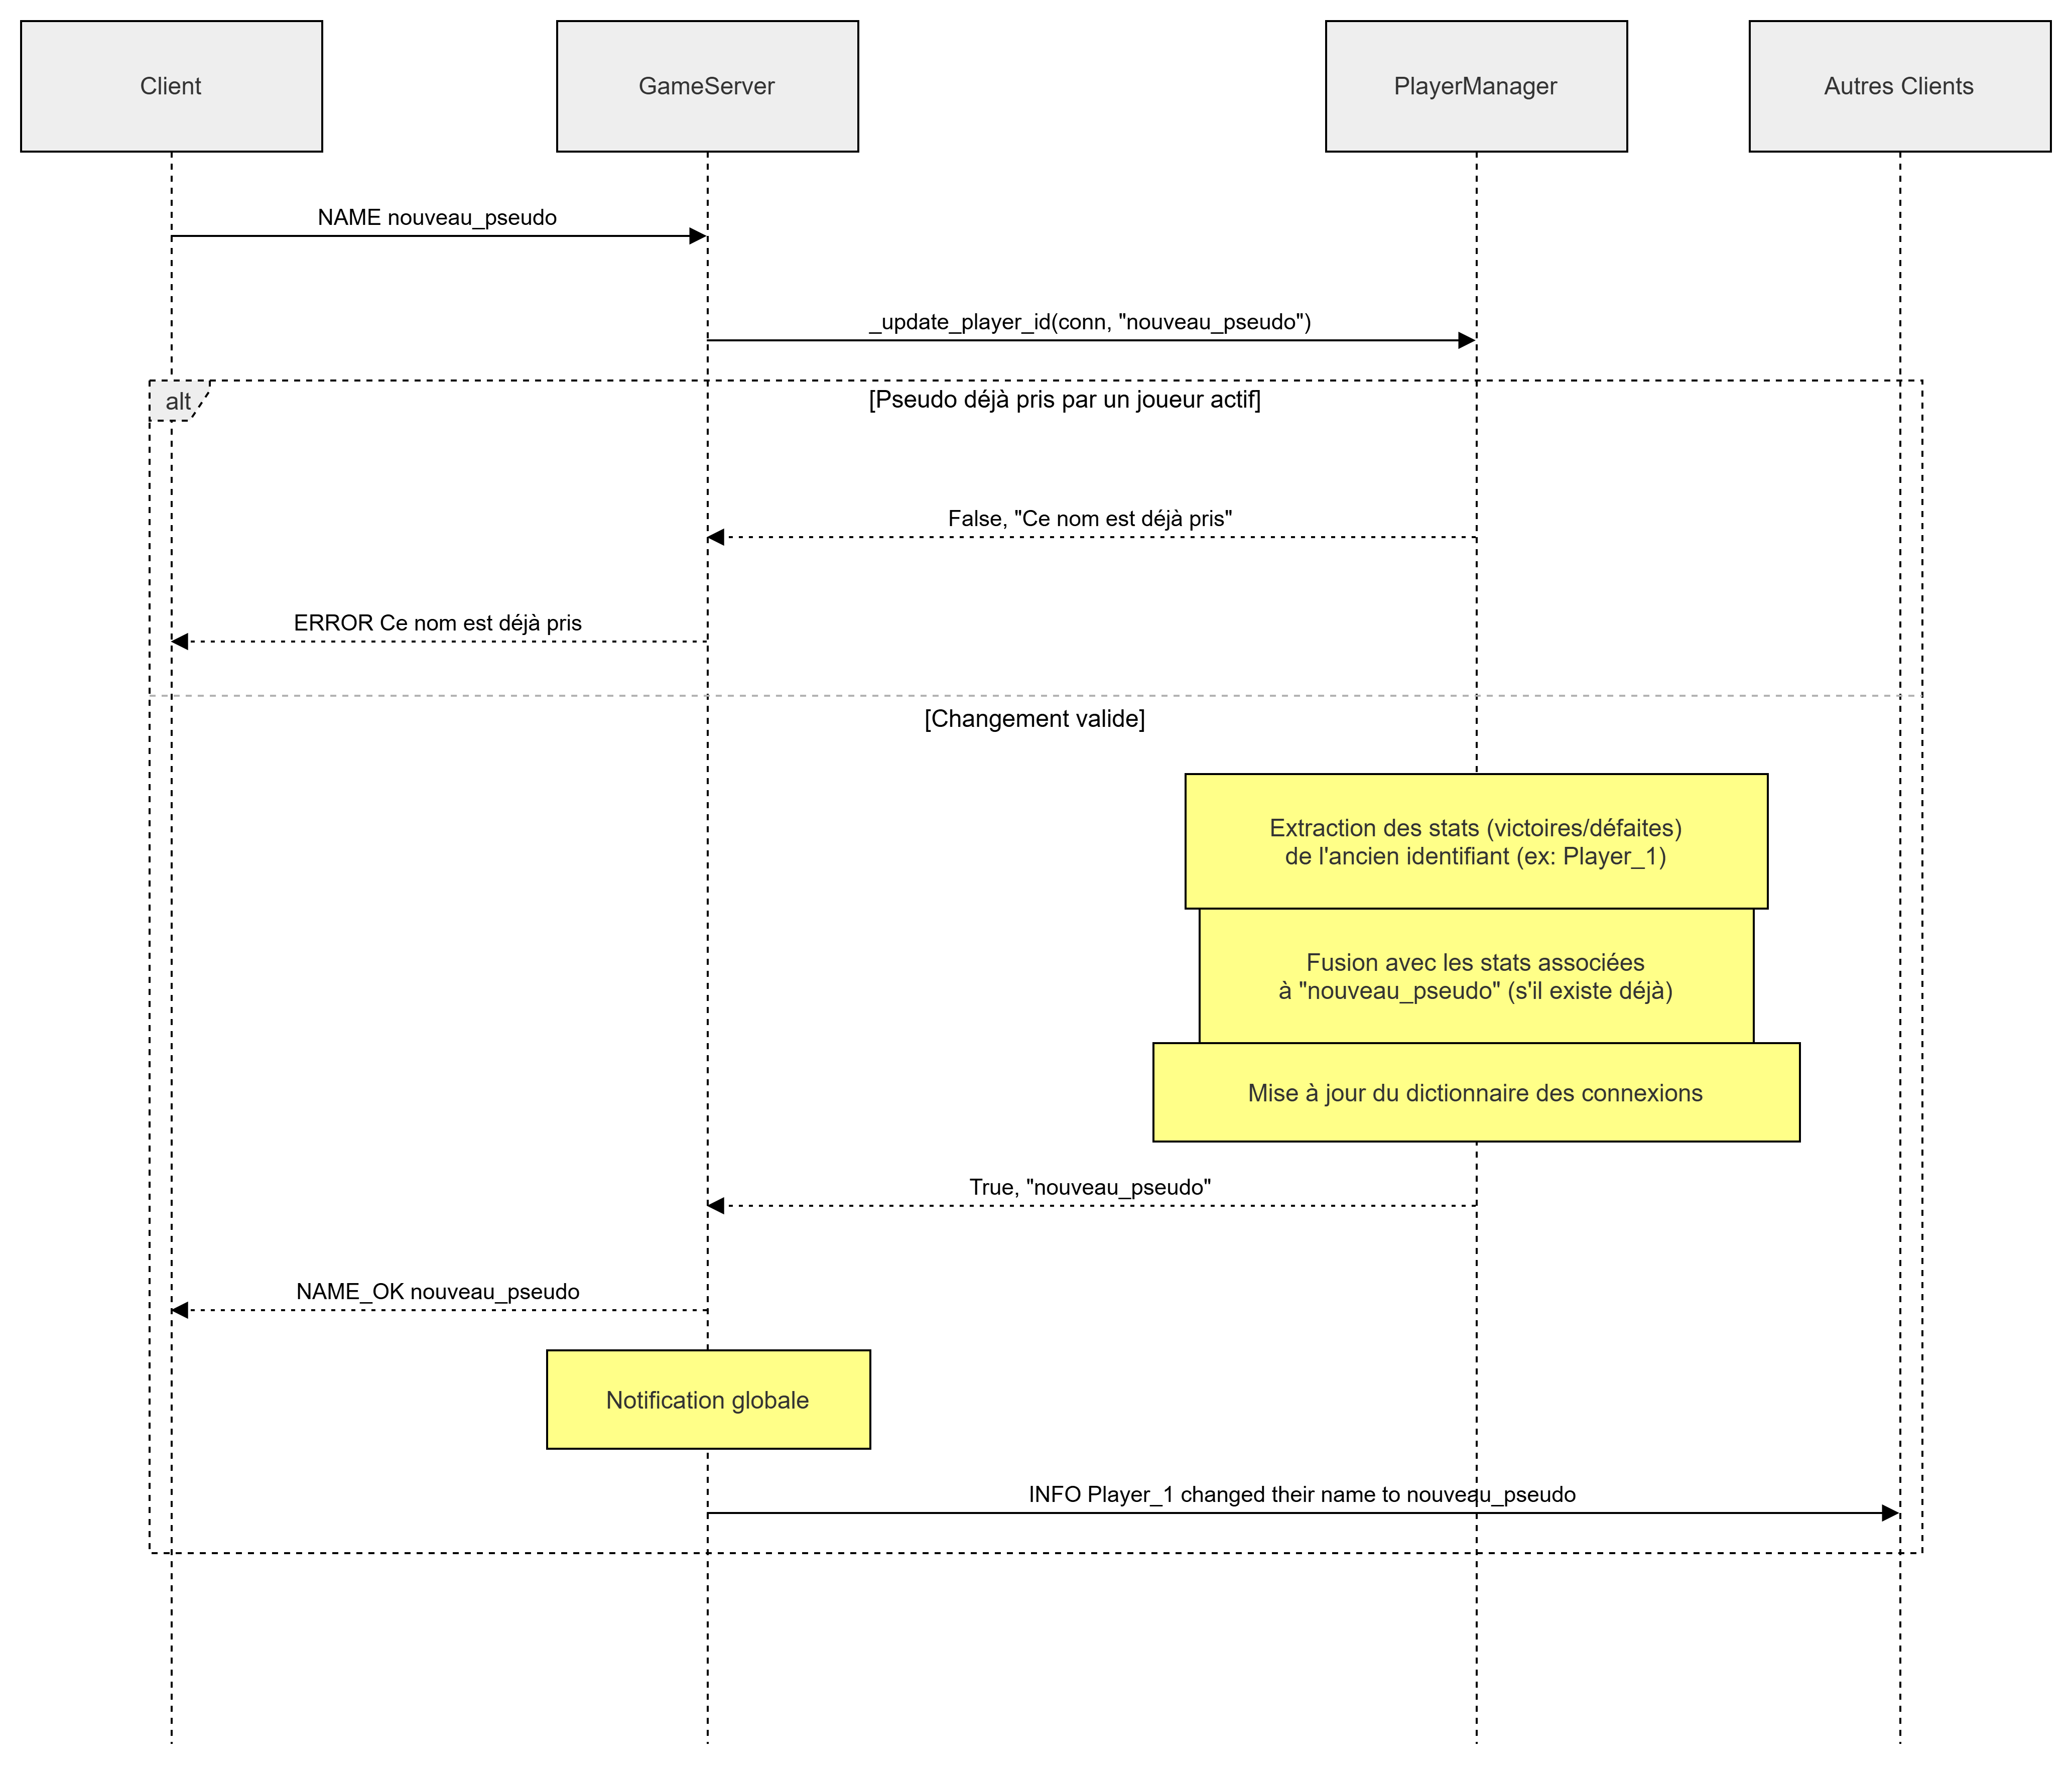
\includegraphics[width=0.7\textwidth]{images/sequence_name_change.png}
    \caption{Diagramme de séquence illustrant la gestion d'un changement de pseudonyme et la fusion des statistiques par le \texttt{PlayerManager}.}
    \label{fig:sequence_name}
\end{figure}

\textbf{3. La classe \texttt{GameRouter} (Arbitrage des parties et invitations)}\\
Le \texttt{GameRouter} implémente la logique de jeu et le système de \textit{matchmaking} côté serveur. Lorsqu'un joueur en invite un autre, la méthode \texttt{handle\_new\_game\_request} entre en action (voir Figure \ref{fig:gamerouter_invitation}). Elle interroge le \texttt{PlayerManager} pour s'assurer que les deux joueurs sont bien en attente (\texttt{idle}). Si c'est le cas, elle modifie leur statut en \texttt{waitgame} et enregistre l'invitation avec un délai d'expiration strict de 5 minutes.
Une fois la partie lancée, le \texttt{GameRouter} valide chaque coup reçu (commande \texttt{MOVE}) via la classe \texttt{GameRules} avant de le retransmettre à l'adversaire, ce qui rend la triche par manipulation du client impossible.

\begin{figure}[H]
    \centering
    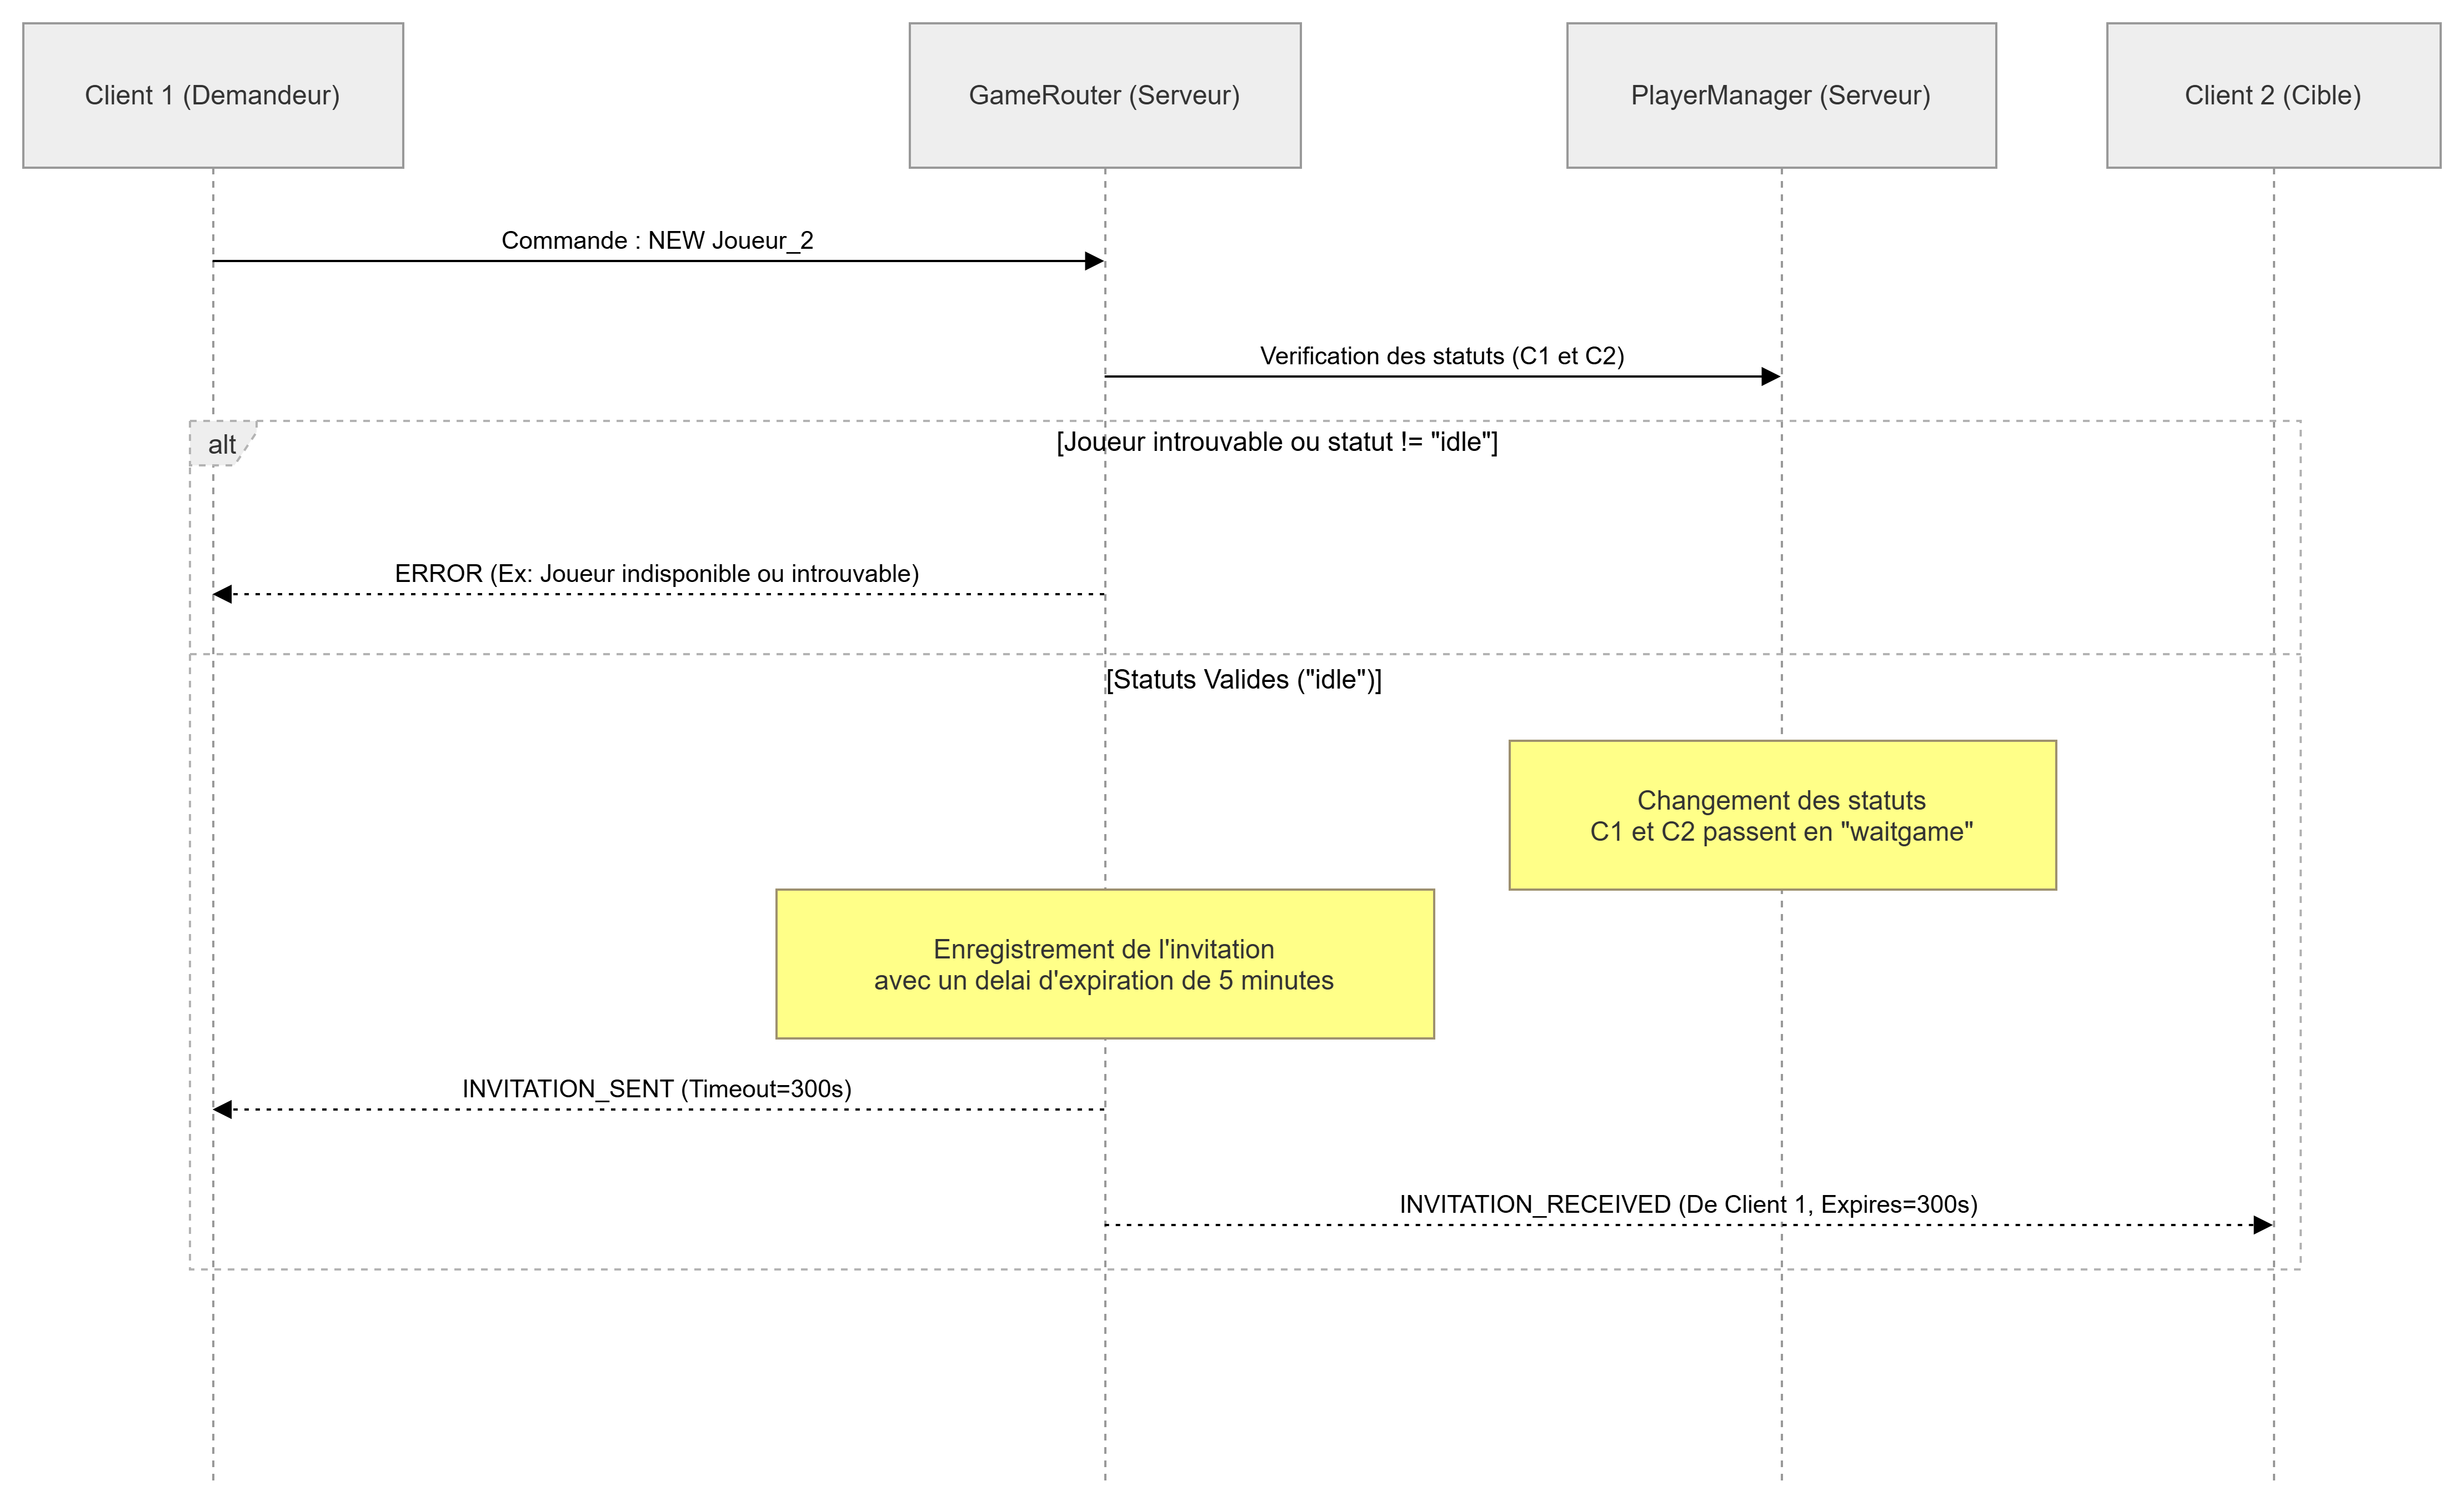
\includegraphics[width=0.7\textwidth]{images/gamerouter_invitation.png}
    \caption{Processus de validation et de création d'une invitation réseau par le \texttt{GameRouter}.}
    \label{fig:gamerouter_invitation}
\end{figure}

\subsection{Justification du Modèle : Multithreading vs Asynchrone pur}

Notre architecture utilise des \textbf{threads} classiques (avec des opérations d'entrée/sortie bloquantes) plutôt que de l'asynchrone pur impliquant une boucle d'événements unique. Ce choix garantit un haut niveau d'équité : si le joueur A subit une forte latence réseau, son thread ralentira, mais le thread du joueur B, totalement indépendant, continuera de traiter ses propres requêtes (demande de score, envois de messages) en temps réel. De plus, cela limite les risques d'attaques par saturation : un client malveillant ne pourra encombrer que son propre fil d'exécution.

\vspace{0.5cm}
\noindent \textbf{Un choix technique pratique :}\\
Ce modèle s'est également imposé pour des raisons d'apprentissage. N'ayant pas de trop de connaissances en programmation asynchrone (\texttt{asyncio}), les propositions d'architecture basées sur ces concepts nous ont paru difficiles à analyser et à déboguer. En revanche, ayant étudié la gestion des processus, des \textit{threads} et de la synchronisation (mutex) en cours d'architecture parallèle, nous avons préféré appliquer ces acquis pour conserver la maîtrise complète de notre code source.

\subsection{L'architecture côté Client : Réception et Interception}

\textbf{1. La classe \texttt{GameClient} et la boucle d'écoute}\\
La difficulté majeure côté client consistait à éviter le gel de l'interface graphique (GUI) ou de la console (CLI) lors de l'attente d'une réponse du serveur. Pour y remédier, le \texttt{GameClient} exécute un thread dédié via la méthode \texttt{\_listen\_loop}. 
Comme illustré par la Figure \ref{fig:listen_loop_client}, cette boucle réceptionne les données TCP. Si elle identifie des messages systèmes cruciaux (\texttt{YOUR\_ID}, \texttt{SYNC\_BOARD}), elle actualise directement les variables du client. Pour tous les autres messages, elle les place dans une file d'attente partagée (\texttt{queue.Queue}), permettant au programme principal de s'actualiser de manière fluide.

\begin{figure}[H]
    \centering
    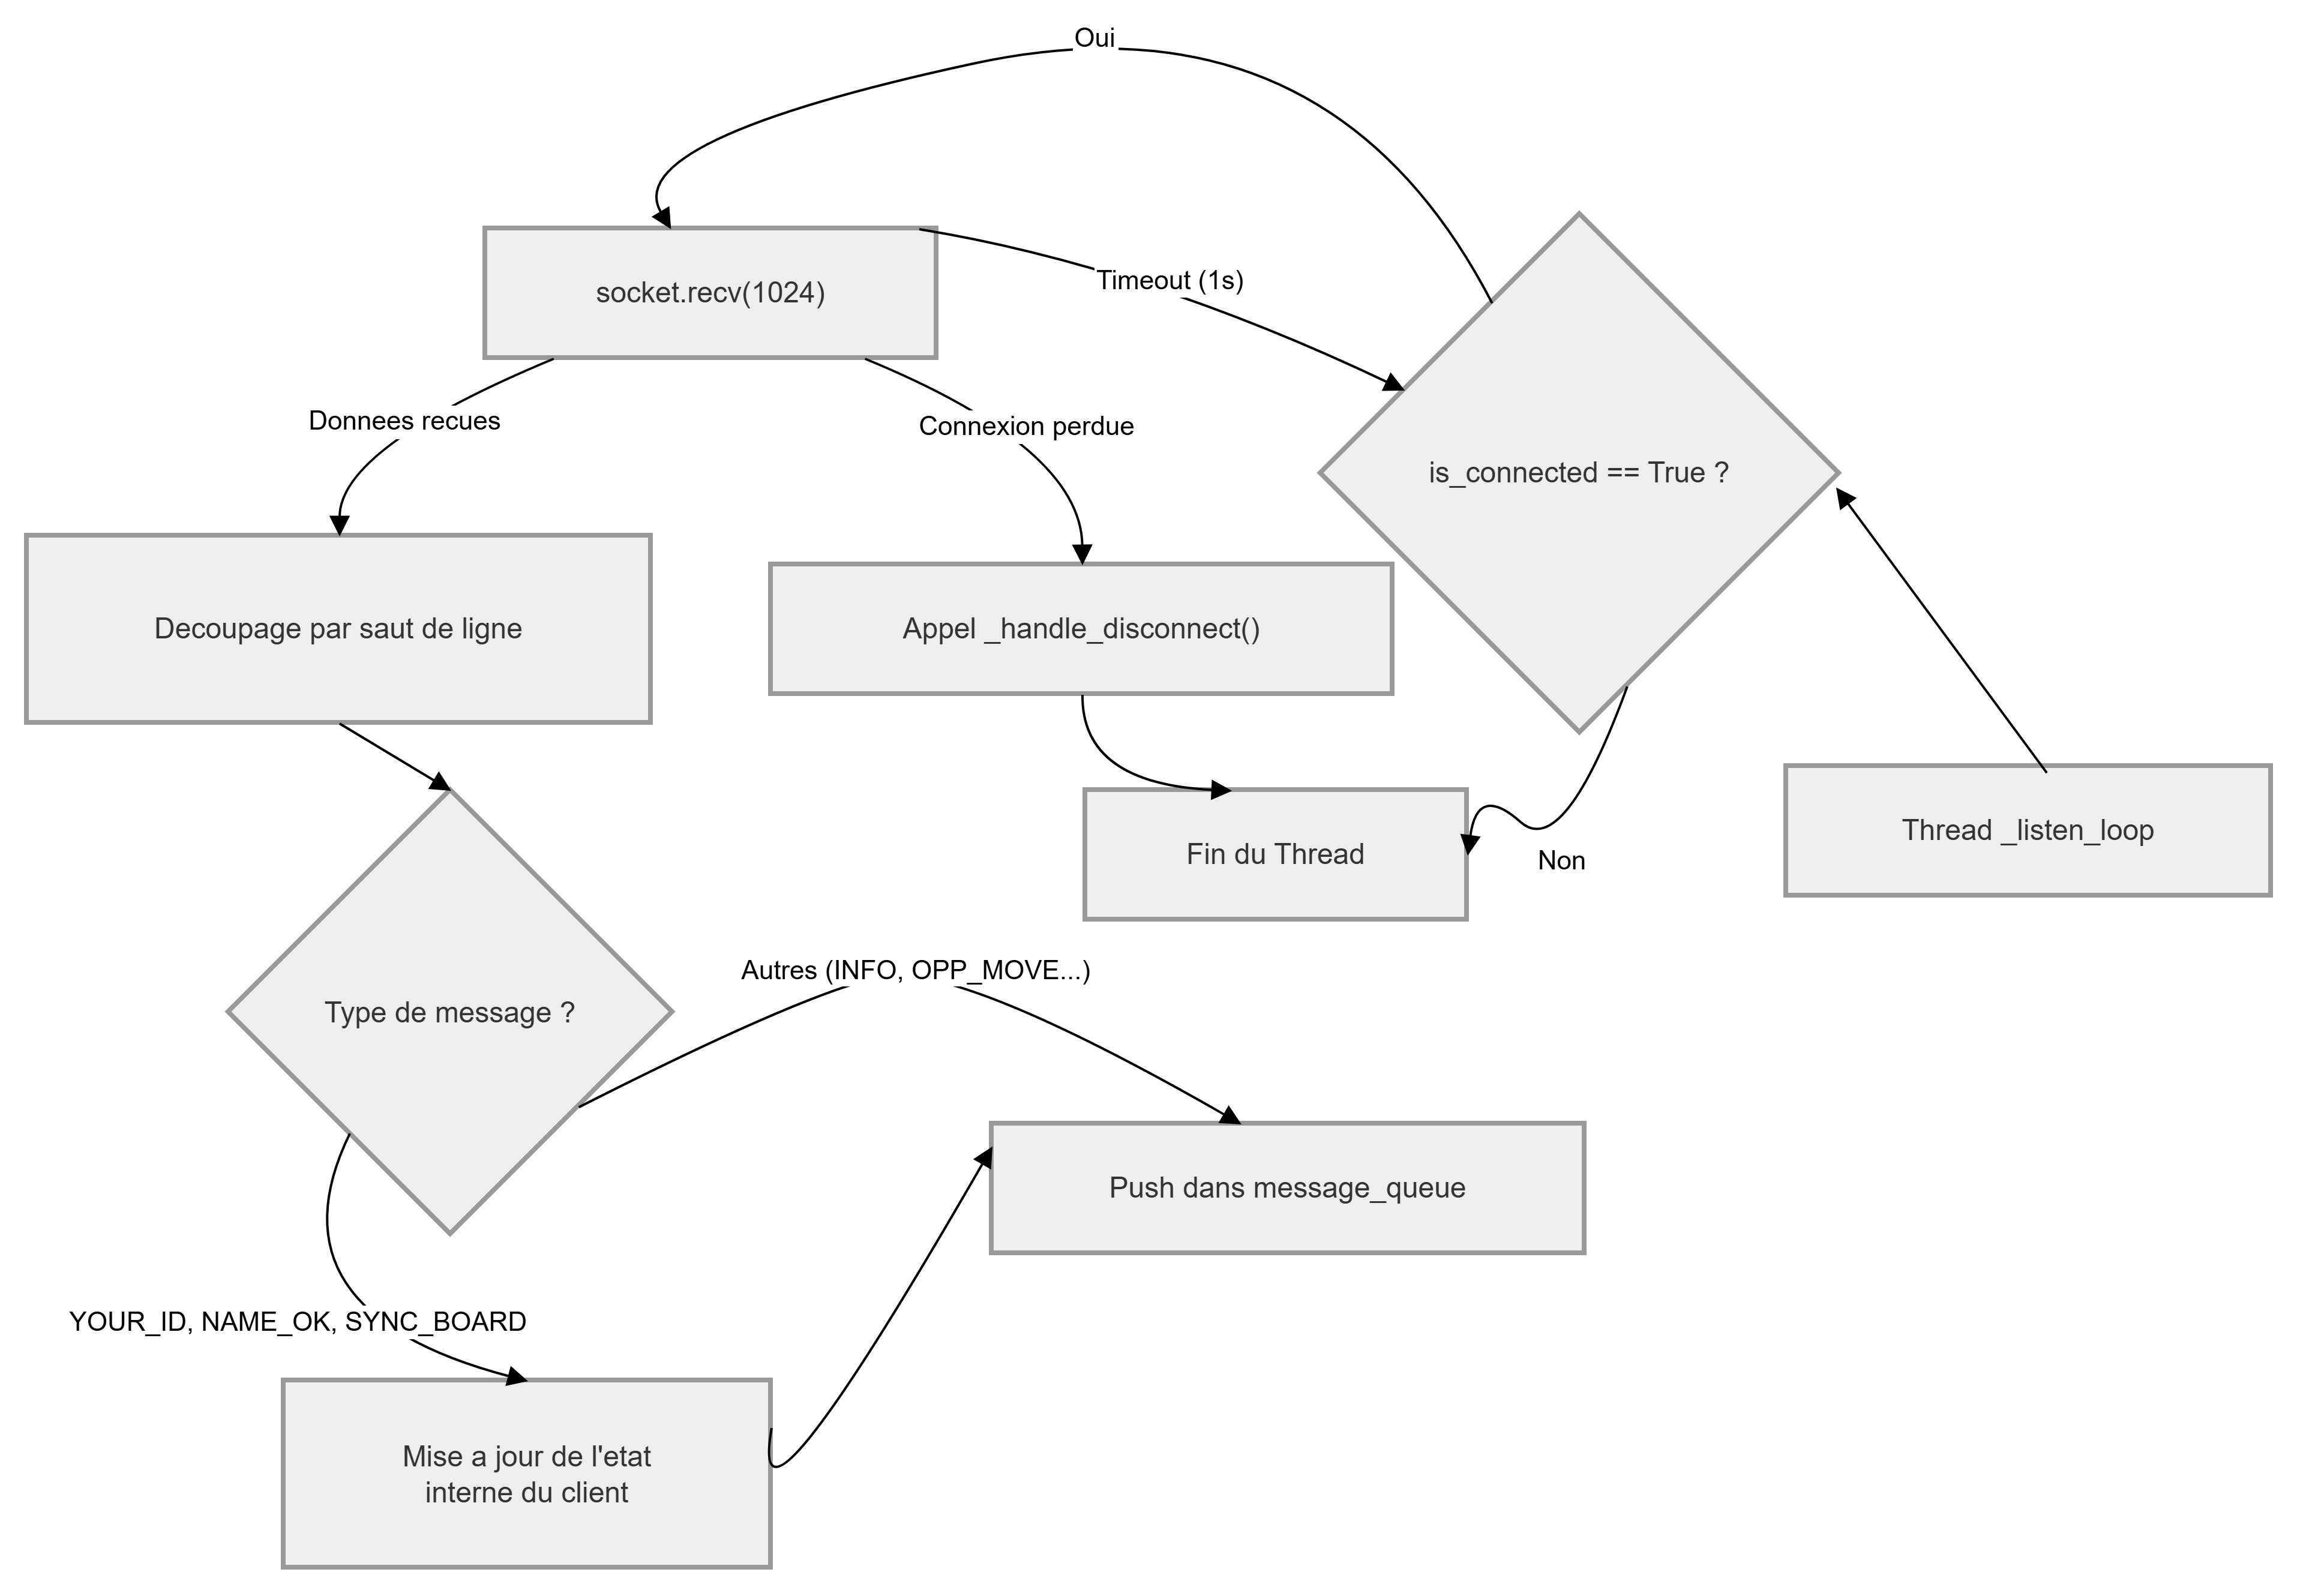
\includegraphics[width=0.55\textwidth]{images/listen_loop_client.png}
    \caption{Logique de la boucle d'écoute (\texttt{\_listen\_loop}) et de sa file d'attente sécurisée.}
    \label{fig:listen_loop_client}
\end{figure}

\textbf{2. La classe \texttt{NetworkPlayer} (Le pont avec le moteur de jeu)}\\
La fonction \texttt{get\_move()} de cette classe devait gérer l'attente du coup adverse sans bloquer l'application. Elle implémente donc une technique de double vérification (\textit{polling} alterné) : elle interroge la file d'attente réseau avec un délai d'expiration très court (0.1 seconde). Si aucun message \texttt{OPPONENT\_MOVE} n'est reçu, elle vérifie si l'utilisateur local n'a pas déclenché une action prioritaire (ex: commande "disconnect" via l'interface). Cela soutient le logiciel, même pendant le tour de l'adversaire (voir Figure \ref{fig:network_player_getmove}).
\begin{figure}[H]
    \centering
    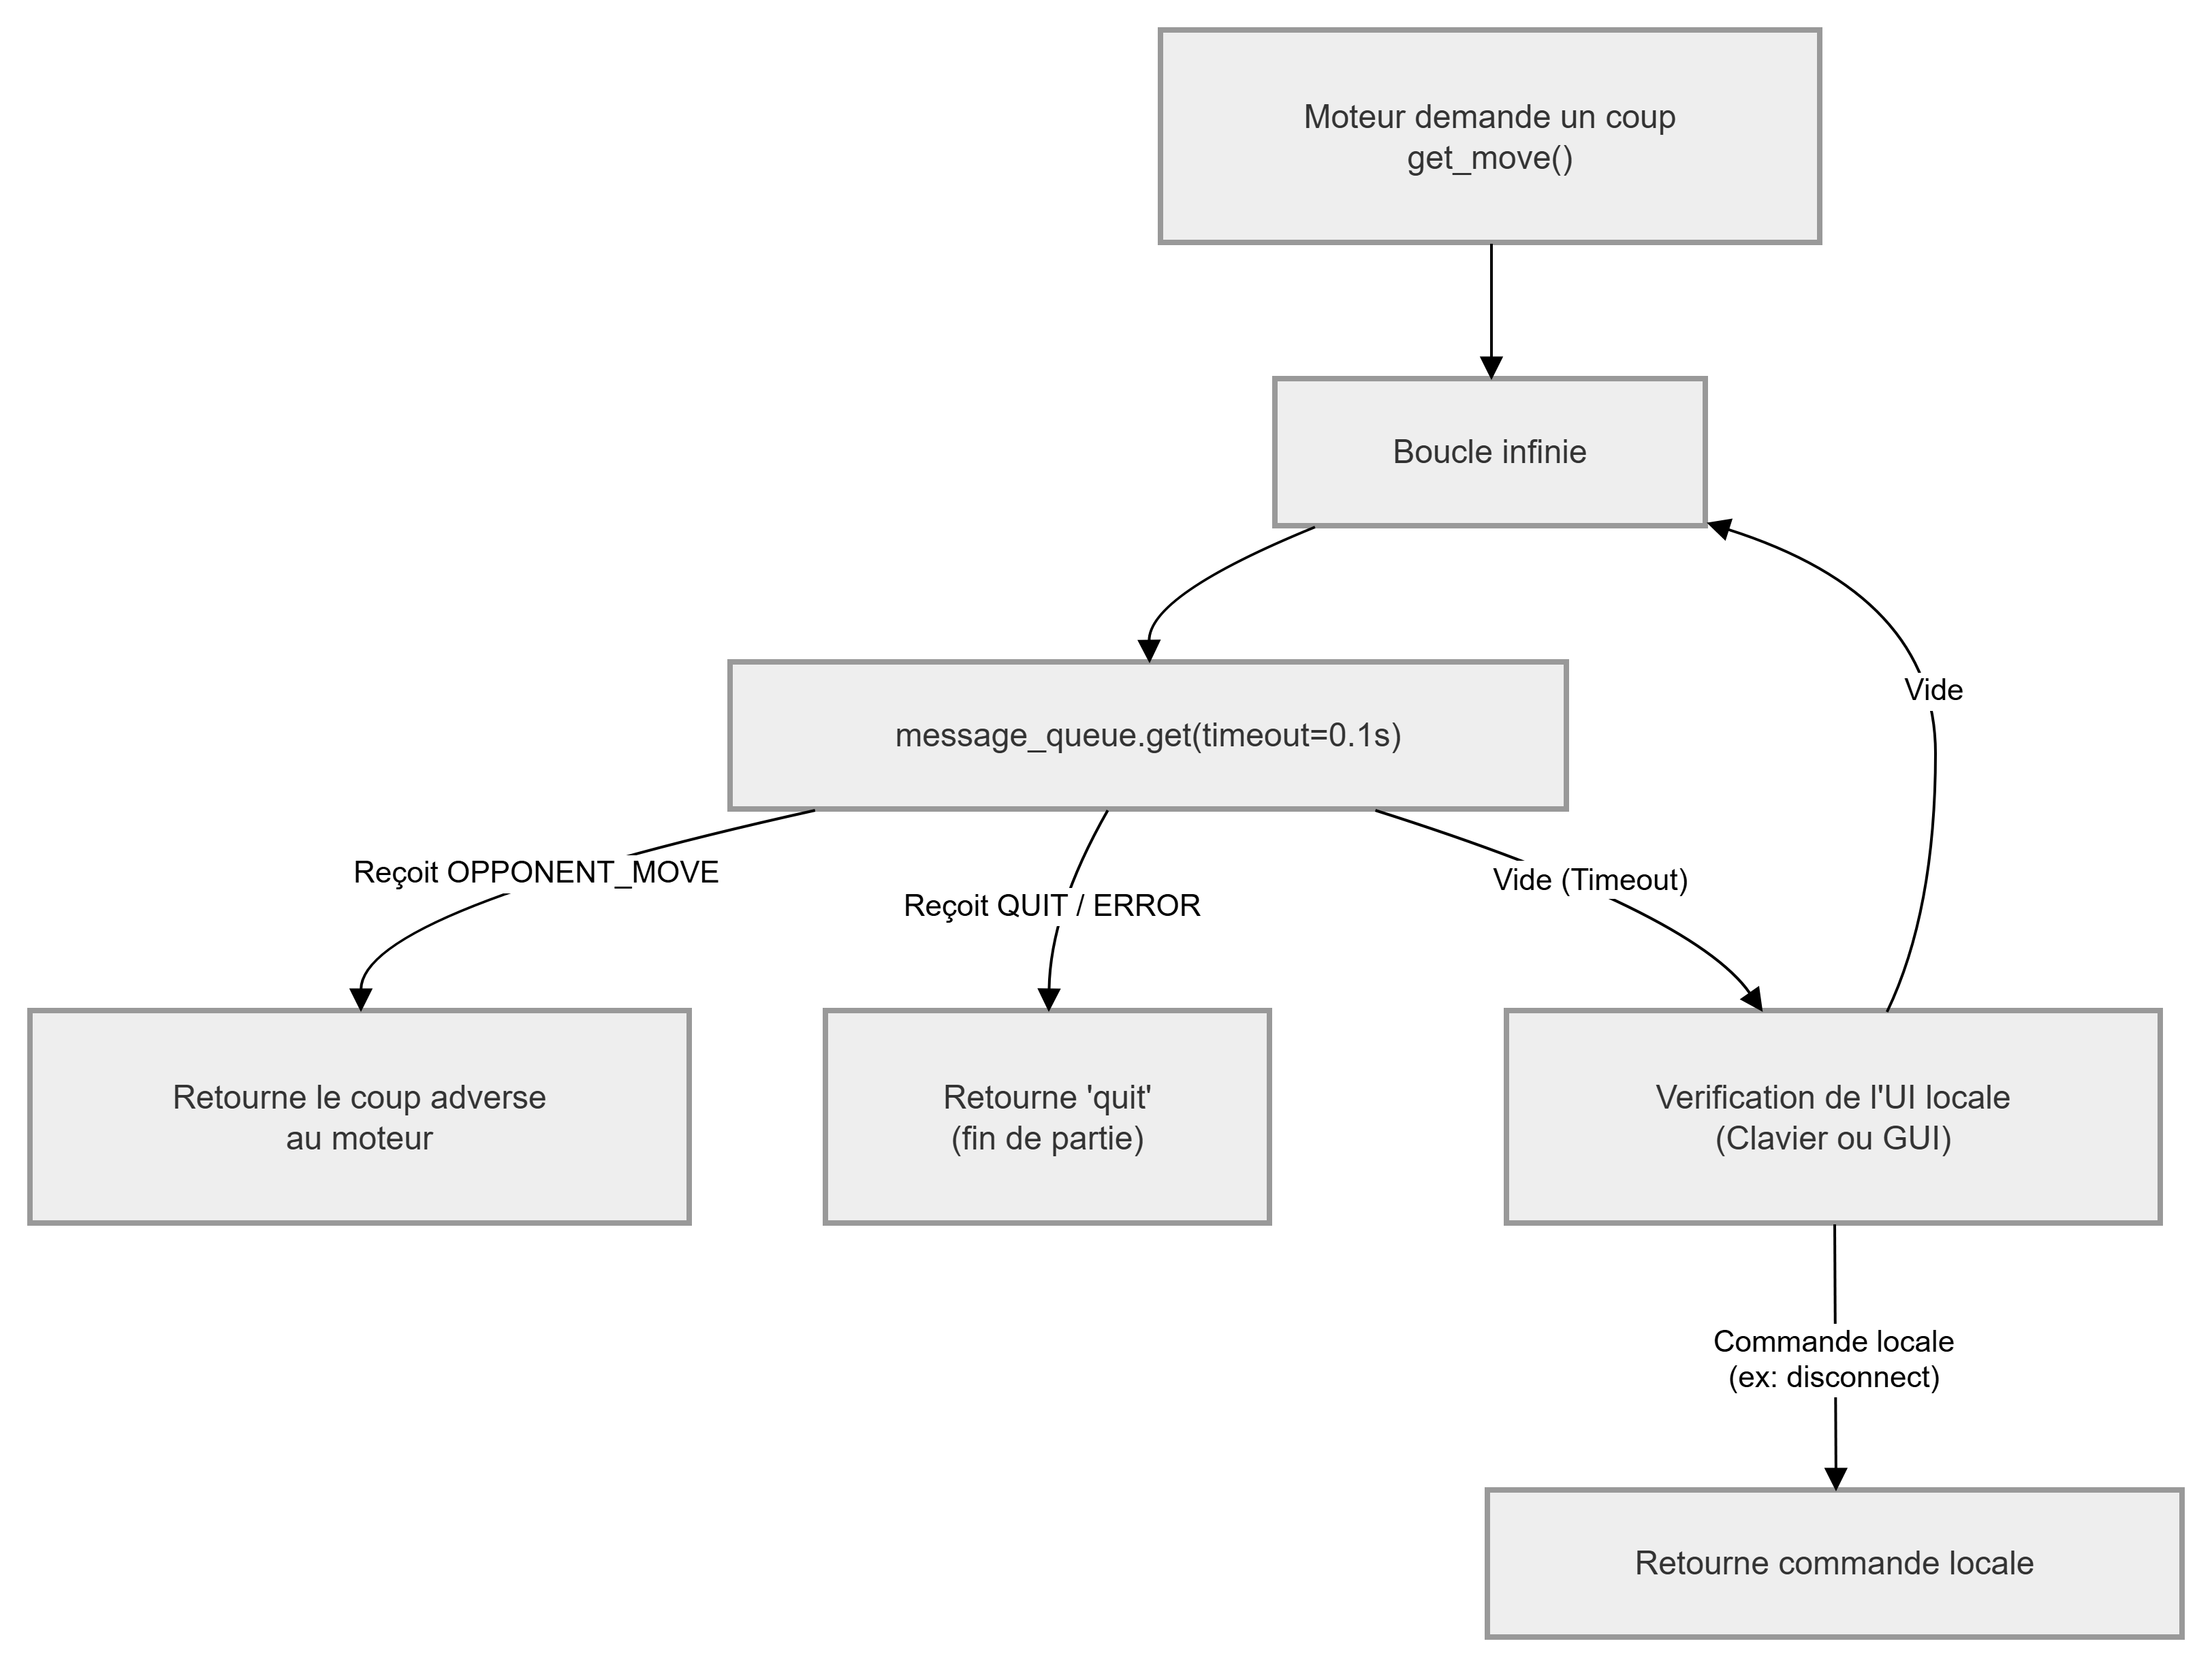
\includegraphics[width=0.65\textwidth]{images/network_player_getmove.png}
    \caption{Mécanique de double écoute (Réseau et Local) dans la méthode \texttt{get\_move()} du \texttt{NetworkPlayer}.}
    \label{fig:network_player_getmove}
\end{figure}

\subsection{Le service de découverte (\texttt{DiscoveryService})}

Pour satisfaire l'exigence \textbf{F38}, nous avons développé un module de découverte automatique basé sur le protocole UDP (Figure \ref{fig:discovery_service}). 

Ce service déploie trois threads parallèles :
\begin{itemize}
    \item \textbf{Le Thread Broadcast (Serveur) :} Il diffuse toutes les 10 secondes une trame JSON (\texttt{PRESENCE}) indiquant le nom du serveur et son port TCP (principe de \textit{Heartbeat}).
    \item \textbf{Le Thread Listener (Client) :} Il écoute le port UDP 12346 en continu et enregistre l'heure de dernière détection de chaque serveur.
    \item \textbf{Le Thread de Nettoyage (Client) :} Il vérifie la liste toutes les 5 secondes. Tout serveur n'ayant pas émis de signal depuis plus de 30 secondes est supprimé, prévenant les tentatives de connexion vers des hôtes hors ligne.
\end{itemize}

\begin{figure}[H]
    \centering
    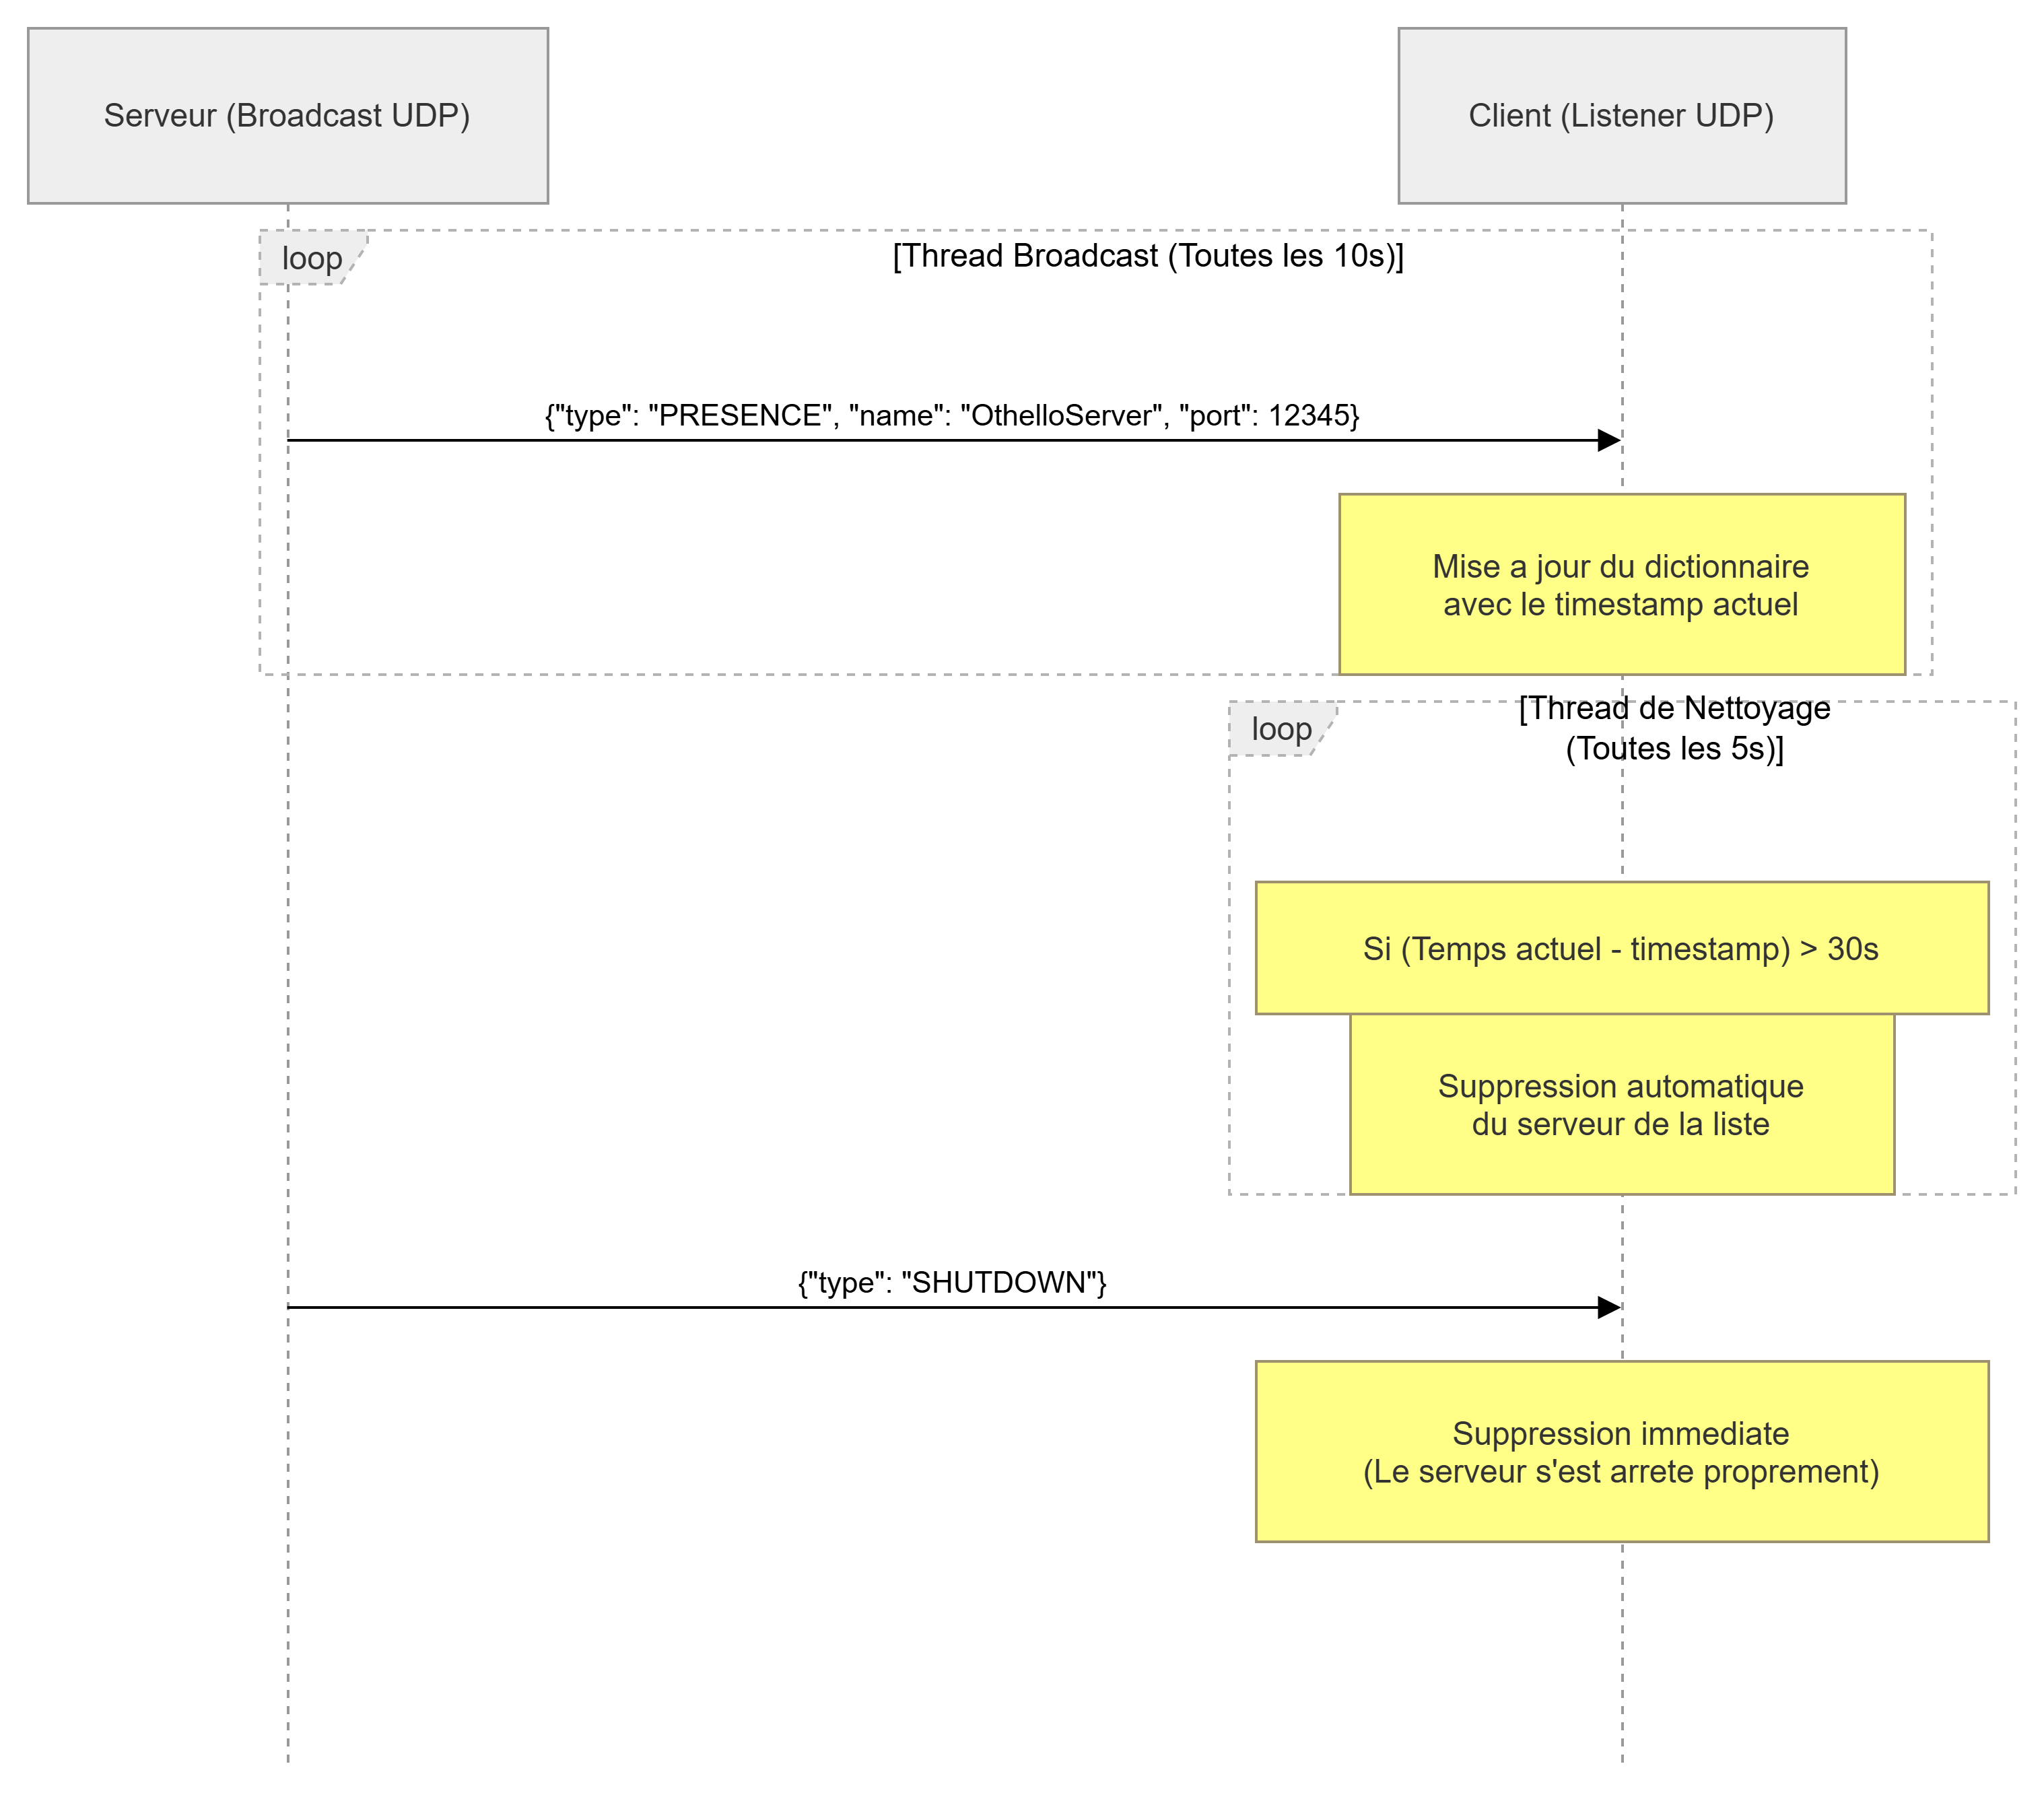
\includegraphics[width=0.4\textwidth]{images/discovery_service.png}
    \caption{Mécanique de signalisation UDP (Heartbeat) du DiscoveryService.}
    \label{fig:discovery_service}
\end{figure}

\subsection{Tolérance aux Pannes et Connexions Fantômes}

La résilience réseau est essentielle. Lorsqu'un joueur perd sa connexion de manière abrupte, le serveur le place dans un registre de déconnexion et lui alloue un délai de grâce de 60 secondes pour se reconnecter.

Néanmoins, une reconnexion immédiate engendre souvent un problème de "connexion fantôme" : l'ancien socket réseau du joueur n'ayant pas encore expiré côté serveur, ce dernier refuse la nouvelle connexion. Notre méthode \texttt{\_remove\_ghost\_connection} pallie ce défaut :

\begin{minted}[frame=single, fontsize=\small]{python}
def _remove_ghost_connection(self, addr):
    """Supprime une ancienne connexion restée active depuis la même IP."""
    client_ip = addr[0]
    with self.lock:
        target_conn = None
        ghost_info = None
        for conn, info in self.players_by_conn.items():
            # Si l'IP correspond et que le profil fantôme est en pleine partie
            if info["addr"][0] == client_ip and info["status"] == "ingame":
                target_conn = conn
                ghost_info = info.copy()
                break

        if target_conn:
            del self.players_by_conn[target_conn]
        return ghost_info
\end{minted}

Une fois l'ancienne instance purgée, le serveur rétablit la session sur le nouveau socket. Il transmet ensuite la commande \texttt{SYNC\_BOARD} contenant l'état des \textit{Bitboards}, permettant au client de rafraîchir son affichage et de reprendre la partie sans interruption visible.

\subsection{Points forts et limites de l'architecture réseau}

Cette architecture présente plusieurs avantages significatifs :
\begin{itemize}
    \item \textbf{Expérience Utilisateur :} La tolérance aux déconnexions (délai de grâce) et la fonctionnalité d'auto-découverte UDP rendent l'application très robuste et facile d'accès sur un réseau local.
    \item \textbf{Sécurité logique :} En centralisant la validation des coups via le \texttt{GameRouter}, il est structurellement impossible pour un client de forcer un mouvement illégal.
\end{itemize}

Cependant, elle possède également des limites inhérentes à sa conception :
\begin{itemize}
    \item \textbf{Scalable :} L'utilisation d'un thread bloquant par client consomme davantage de ressources système (mémoire et changement de contexte processeur) qu'un modèle asynchrone pur. Si cette approche est excellente pour quelques dizaines de joueurs, elle peinerait à gérer des milliers de connexions simultanées sur un serveur modeste.
    \item \textbf{Absence de chiffrement :} Les échanges TCP et UDP transitent actuellement en texte clair. Dans l'éventualité d'un déploiement sur Internet (et non en réseau local), il serait nécessaire d'encapsuler les sockets TCP dans un contexte TLS (\texttt{ssl.wrap\_socket}) pour éviter l'interception des données.
\end{itemize}
\section{Revue critique du projet}

Nous allons maintenant se concentrer sur la revue critique de l'application Othello. L'objectif est de comparer notre logiciel Othello fini aux exigences du cahier des charges, d'analyser les performances et les limites de notre production, et d'identifier les axes d'amélioration potentiels.

\subsection{Ce qui a été accompli : Un respect rigoureux du cahier des charges}

Le projet répond parfaitement aux attentes techniques. Côté architecture, nous avons découpé chaque composant en modules indépendants, ce qui rend le code beaucoup plus clair et facile à maintenir.

\subsubsection{Moteur de jeu et représentation par Bitboards (F26, F27 \cite{OthelloSpecs2025})}
L'une des parties les plus importantes du projet réside dans l'intégration de la structure de données en \textit{bitboards}. Conformément à l'exigence \textbf{F26} \cite{OthelloSpecs2025}), l'état du plateau n'est pas stocké dans une matrice bidimensionnelle, mais via deux entiers 64-bits (un pour les noirs, un pour les blancs) encapsulés dans la classe \texttt{GameState}.
Les algorithmes manipulant ces structures (feature \textbf{F27} \cite{OthelloSpecs2025}) exploitent les décalages binaires et les masques. Par exemple, le calcul de la légalité d'un coup dans \texttt{game\_rules.py} s'effectue en temps constant grâce à la vérification qu'une case est vide via un masque binaire:
\begin{minted}[frame=single, fontsize=\small]{python}
# Vérification case vide via masquage binaire
index = (row * size) + col
mask = 1 << index
if (player_bb | opponent_bb) & mask:
    return False
\end{minted}
Cette implémentation garantit une constance des états lors de l'exploration arborescente de l'intelligence artificielle.

\subsection{Écarts au cahier des charges : Ce qui n'a pas été fait}
\subsubsection{Serveur asynchrone et système d'invitations (F39) \cite{OthelloSpecs2025}}
Le cahier des charges demande un système complexe de gestion d'état des joueurs sur le serveur réseau (\texttt{idle}, \texttt{away}, \texttt{waitgame}, \texttt{ingame}) ainsi que des \textit{timeouts} d'invitations stricts de 5 minutes. Actuellement, la création de processus démons repose sur la fonction système \texttt{os.fork()}, ce qui limite la portabilité logicielle (incompatible sous Windows) et restreint la flexibilité requise pour implémenter une machine à états asynchrone complexe telle que demandée par l'exigence \textbf{F40}.

\subsection{Analyse des performances et Cas Limites}

La contrainte \textbf{F1.8} exige la mesure et la documentation des performances, particulièrement dans les cas limites.

\subsubsection{Analyse des résultats IA}
L'entraînement de ce modèle a permis d'atteindre une précision de 78\% sur le jeu de test. L'analyse de la courbe d'apprentissage révèle que les lignes d'entraînement et de validation se rapprochent pour former ce qu'on appelle un "entonnoir" (voir Figure \ref{fig:rf_learning_curve}). De plus, le graphique montre que l'ajout de données supplémentaires au-delà d'un million d'exemples n'apporterait qu'un gain de performance marginal, validant ainsi la taille de notre dataset.

La dynamique contre-intuitive de ces courbes (baisse continue de la précision d'entraînement) s'explique par le concept de \textit{capacité du modèle}. En fixant \verb|max_leaf_nodes=25000|, nous avons délibérément bridé la mémoire de l'algorithme via un processus de régularisation. Pour illustrer ce principe, imaginons un étudiant disposant d'un petit carnet de notes de taille fixe. S'il ne doit résumer que 5 ouvrages (équivalent à nos 200 000 premiers exemples), il a suffisamment d'espace pour les mémoriser presque mot pour mot. Cela explique l'excellente précision initiale de 94\% en entraînement, qui n'est en réalité que le fruit d'un apprentissage par cœur incapable de généraliser. À l'inverse, lorsqu'il doit condenser 50 ouvrages dans ce même carnet (notre palier à un million d'exemples), il est contraint de cesser la mémorisation brute pour en extraire uniquement les concepts stratégiques fondamentaux. L'algorithme commet logiquement plus d'erreurs sur ses propres données d'entraînement (chute à 84\%), mais acquiert une compréhension globale beaucoup plus solide face à l'inconnu, propulsant ainsi la précision de validation à 78\%. C’est la preuve absolue que le modèle généralise bien et évite le surapprentissage (\textit{overfitting}).

\begin{figure}[H]
    \centering
    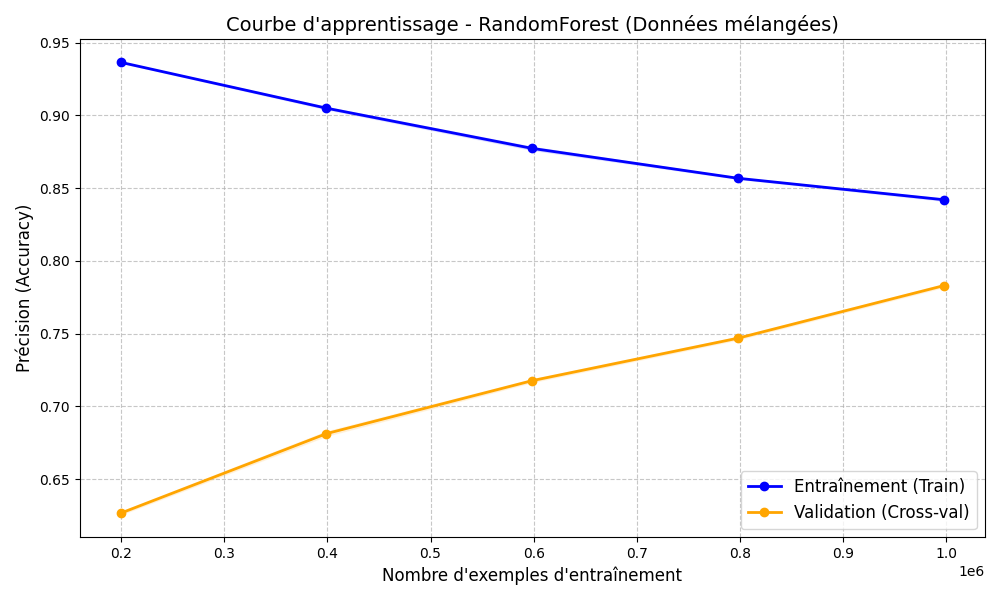
\includegraphics[width=0.60\textwidth]{images/rf_learning_curve.png}
    \caption{Courbe d'apprentissage du modèle Random Forest illustrant la convergence des scores.}
    \label{fig:rf_learning_curve}
\end{figure}

\subsubsection{Bilan des performances CNN}
L'architecture CNN a permis de franchir un nouveau palier avec une précision évaluée à plus de 81,8\% sur les données de test inédites. La Figure \ref{fig:cnn_learning_curves} illustre la stabilité de l'apprentissage et l'intervention de l'arrêt précoce avant l'effondrement de la perte de validation. Ce score valide notre démarche : bien qu'un jeu à information parfaite impliquerait une précision théorique de 100\% (irréalisable sans mémoriser l'arbre complet du jeu), un score approchant les 82\% témoigne d'une excellente capacité de généralisation et d'abstraction des concepts stratégiques de l'Othello.

\begin{figure}[H]
    \centering
    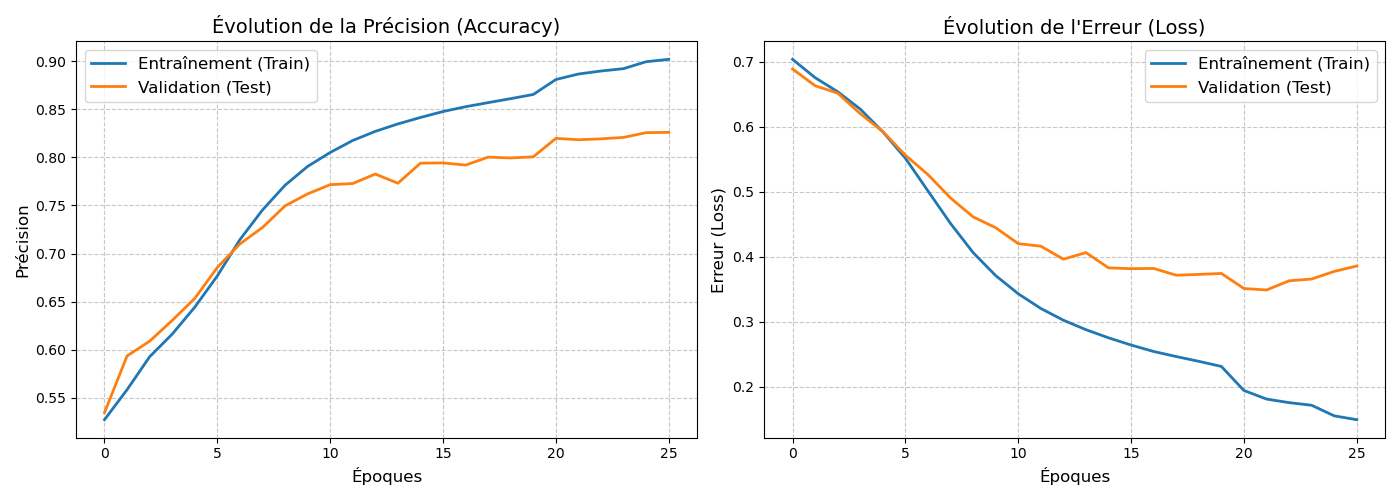
\includegraphics[width=0.8\textwidth]{images/learning_curves.png}
    \caption{Évolution de la précision (Accuracy) et de la perte (Loss) durant l'entraînement du réseau convolutif.}
    \label{fig:cnn_learning_curves}
\end{figure}

\subsubsection{Évaluation empirique : Tournoi des Intelligences Artificielles}

Afin de confronter nos hypothèses théoriques à la réalité algorithmique de notre moteur, nous avons développé un script d'automatisation de tournoi. Ce script coordonne des affrontements directs entre nos différentes implémentations d'IA sur un échantillon de parties, en leur allouant un temps de réflexion strictement identique (1 seconde par coup). L'intégration du MCTS classique (fonction de sélection UCB1 avec simulations aléatoires) permet d'établir une hiérarchie complète de nos agents.

\begin{table}[H]
    \centering
    \renewcommand{\arraystretch}{1.2}
    \begin{tabular}{|l|c|c|c|}
        \hline
        \textbf{Affiche du Duel (Noirs vs Blancs)}          & \textbf{Victoires IA 1} & \textbf{Victoires IA 2} \\
        \hline
        Minimax (Bitboards) vs MCTS (Deep Learning - CNN)   & 100\%                   & 0\%                     \\
        \hline
        Minimax (Bitboards) vs MCTS (Machine Learning - RF) & 85\%                    & 15\%                    \\
        \hline
        Minimax (Bitboards) vs MCTS classique (UCB1)        & 0\%                     & 100\%                   \\
        \hline
        MCTS classique (UCB1) vs MCTS (Deep Learning)       & 100\%                   & 0\%                     \\
        \hline
        MCTS (Machine Learning) vs MCTS (Deep Learning)     & 80\%                    & 20\%                    \\
        \hline
        MCTS (Machine Learning) vs MCTS classique (UCB1)    & 50\%                    & 50\%                    \\
        \hline
    \end{tabular}
    \caption{Résultats statistiques finaux des 10 confrontations entre les agents (Temps imparti : 1s / coup).}
    \label{tab:ia_tournament_complet}
\end{table}

\paragraph{Analyse transversale des résultats de la confrontation}
Ces statistiques correspondent parfaitement notre analyse de l'architecture logicielle et mettent en lumière la hiérarchie des algorithmes face à la contrainte du temps réel. Le paradoxe apparent de ces résultats confirme une règle fondamentale : \textbf{le volume d'exploration arborescente prime sur la qualité de l'évaluation unitaire lorsque le temps est contraint}.

Bien que le réseau convolutif (CNN) soit le modèle le plus précis pour évaluer un plateau (81,8\% de précision), la latence matérielle de l'appel aux bibliothèques Keras (\textit{overhead} d'inférence unitaire) bride drastiquement sa capacité à itérer dans l'arbre MCTS. Conséquence directe : il s'incline lourdement face à des algorithmes plus rudimentaires mais plus rapides, y compris face au MCTS classique (UCB1) qui, bien que jouant ses simulations de manière totalement aléatoire, effectue des milliers de tirages là où le CNN n'en réalise que quelques dizaines.

Le modèle \textit{Random Forest} s'impose comme le meilleur compromis parmi les approches statistiques : sa structure d'arbre décisionnel s'exécute sur CPU avec une légèreté suffisante pour guider efficacement le MCTS, lui permettant de surpasser à la fois le CNN (par le volume d'exploration) et l'UCB1 classique (par la pertinence de son évaluation heuristique).

Enfin, le \textit{Minimax} s'affirme comme le vainqueur absolu du tournoi. La rapidité d'exécution des \textit{Bitboards} permet d'anticiper 5 à 7 coups à l'avance, une profondeur d'analyse que les modèles d'apprentissage ne peuvent atteindre dans le temps imparti. Cela confirme que pour un jeu déterministe comme Othello, le calcul exact et optimisé l'emporte toujours sur l'estimation probabiliste.

\subsubsection{Conclusion sur les modèles décisionnels et niveaux de difficulté}

L'évaluation empirique de ces différentes intelligences artificielles nous permet finalement de hiérarchiser nos algorithmes et d'offrir des niveaux de difficulté pertinents au joueur.

Le niveau \textbf{Facile} s'appuie logiquement sur l'algorithme Random Forest (MCTS). Bien qu'il saisisse les concepts primordiaux de l'Othello, sa limitation à l'exploration MCTS en temps contraint le pousse parfois à réaliser des erreurs tactiques à moyen terme. Il incarne l'adversaire idéal pour permettre à un joueur débutant de s'exercer et de gagner avec une difficulté modérée.

Le niveau \textbf{Moyen} tire avantage du réseau convolutif profond (CNN) ou du MCTS classique avec UCB1. L'approche spatiale du CNN lui confère une solide réflexion stratégique. Cependant, bridé par son temps d'inférence face aux millions de calculs du Minimax, il offre une fenêtre de tir tactique dont un joueur aguerri pourra tirer profit dans les séquences combinatoires de fin de partie.

Le niveau \textbf{Difficile} est sans conteste dominé par le classique algorithme \textbf{Minimax} perfectionné par sa recherche par Bitboards. Sa suprématie provient de sa recherche exhaustive et ininterrompue, lui permettant l'anticipation redoutable et systématisée de plus de 5 tours dans une limite temporelle infime. Évaluant avec précision la stabilité de chaque encadrement de pions, il punit de façon mathématique toutes les imprécisions d'un adversaire, s'imposant ainsi comme le défi ultime de notre écosystème d'Othello.

\subsubsection{Le goulot d'étranglement du Machine Learning}
L'intégration de Keras/Scikit-learn dans l'arbre MCTS (exigence \textbf{F37} \cite{OthelloSpecs2025})) s'avère être un goulot d'étranglement de performance majeur. Dans la méthode \texttt{ml\_dl\_selection}, l'inférence est appelée de manière unitaire pour évaluer la probabilité de victoire à chaque sélection de nœud :
\begin{minted}[frame=single, fontsize=\small]{python}
ml_input = np.array(grid).reshape(1, 12, 12, 1)
proba = self.model.predict(ml_input, verbose=0)[0][0]

\end{minted}
Dans des cas limites où le temps de réflexion est de l'ordre d'une seconde, le surcoût (\textit{overhead}) généré par l'appel à \texttt{model.predict} empêche le MCTS de réaliser suffisamment d'itérations (rollouts), rendant paradoxalement l'IA basée sur le ML/DL moins performante qu'un simple Minimax avec heuristique basique.

\subsubsection{Prédiction adaptative de la profondeur}

Pour optimiser l'utilisation du temps imparti, la méthode \texttt{predict\_depth} estime la profondeur de recherche maximale possible. On a développé cette formule en se basant sur la nature exponentielle de l'arbre de recherche, où le volume de calcul dépend directement du facteur de branchement du plateau.

Le modèle repose sur deux constantes mesurées expérimentalement par benchmarks :
\begin{itemize}
    \item $t_{base} = 0.0002$ : le temps initial requis pour une recherche de base.
    \item $g = 3.08$ : le facteur de croissance moyen du temps de calcul à chaque incrément de profondeur.
\end{itemize}

Le temps de recherche estimé $T(d)$ en fonction de la profondeur $d$ suit la loi :
\[ T(d) = t_{base} \times g^{d-1} \]

En isolant $d$ pour obtenir la profondeur à partir d'une limite de temps $T$, on obtient la formule de prédiction :
\[ d = 1 + \frac{\ln(T / t_{base})}{\ln(g)} \]

Le code implémente cette logique tout en appliquant une correction selon le facteur de branchement actuel $b$ (nombre de coups possibles) pour compenser les variations de densité du plateau, ainsi qu'une marge de sécurité finale :

\begin{minted}[frame=single, fontsize=\small]{python}
# Constantes empiriques (calibrage machine)
base_time = 0.0002
growth = 3.08

# Calcul de la profondeur théorique brute
depth = 1 + math.log(time_limit / base_time) / math.log(growth)

# Correction selon le facteur de branchement (base moyenne de 6 coups)
depth -= math.log(branching_factor / 6) / math.log(growth)

# Résultat final avec marge de sécurité
final_depth = max(1, int(depth) - 1)
\end{minted}

\textbf{Limites et imprécisions de l'approche :}
Malgré son efficacité pratique, cette méthode souffre d'une forte dépendance à l'architecture matérielle hôte : 
des constantes calibrées sur un processeur récent seront totalement inadaptées sur une machine plus lente (ex: Raspberry Pi). 
De plus, l'élagage alpha-beta rend la croissance de l'arbre irrégulière ; cette approche purement statistique ne peut donc garantir un respect strict du temps 
imparti et nécessite une gestion robuste des interruptions (timeouts) en complément.
\subsubsection{Analyse des Performances des algo IA}
Malgré l'optimisation par bitboards, le langage Python demeure le principal goulot d'étranglement pour la performance du moteur. 
Une profondeur de recherche située entre 6 et 8 niveaux représente généralement la limite pour maintenir un jeu fluide, alors que des implémentations en langages compilés comme le C++ atteindraient facilement des profondeurs plus élevées. L'efficacité de l'élagage Alpha-Beta est également limitée par l'absence d'un système d'ordonnancement des coups. Sans un tri préalable testant les coups à fort potentiel comme les coins, le nombre de branches du jeu réellement coupées reste suboptimal. Par ailleurs, l'algorithme MCTS souffre particulièrement de la lenteur de l'interpréteur Python, car il repose sur des milliers de simulations aléatoires successives. Cela rend souvent cette approche moins compétitive que le Minimax pour un budget de temps identique sur une machine standard.

\subsubsection{Performances et réactivité de l'Interface Graphique (GUI)}
Pour garantir que l'interface graphique ne fasse pas crasher le système nous avons essayez d'implémenter plusieurs optimisations.

Un \textbf{rendu optimisé} avec une interface qui ne détruit et ne recrée pas les boutons de la grille GTK à chaque tour. Elle se contente de mettre 
à jour les classes CSS (\texttt{piece-X}, \texttt{piece-O}, \texttt{legal-move}), allégeant ainsi la charge sur le moteur de rendu.
Une \textbf{interface non-bloquante (Thread-Safety)} grâce à une architecture basée sur des files d'attente (\texttt{queue.Queue}), 
le thread principal de GTK n'est jamais bloqué par les calculs lourds de l'IA ou les requêtes réseau. Les événements asynchrones sont traités par lots.
Une \textbf{Gestion des cas limites }, l'interface possède des verrous stricts contre le spam de clics (les actions hors-tour sont ignorées). 
De plus, L'appli ne plante pas si les paquets réseau arrivent de manière asynchrone ou avec du retard lorsque des fenêtres contextuelles (Lobby, Join) 
viennent d'être fermées par l'utilisateur, ignorant silencieusement les événements orphelins sans faire crasher l'application.


\subsection{Vulnérabilités, Bugs et Limitations structurelles}

L'exigence \textbf{F1.7} stipule qu'aucun bug menant à un crash ne doit être présent. apres analyse de notre projet nous n'avons decouverts aucun bugs menant à un crash de notre jeu othello cependant nous avons identifié plusieurs vulnérabilités et limitations structurelles qui pourraient potentiellement conduire à des comportements indésirables.

Il y a un\textbf{terminaison brutale en cas d'impasse (Hard Exit)}dans le module IA si l'agent est invoqué sur un plateau sans aucun coup légal détecté 
(scénario théoriquement impossible en jeu normal, mais possible via la manipulation du fichier de sauvegarde), la fonction de repli \texttt{random\_move} 
affiche un message de bug et force l'arrêt du programme via un appel à \texttt{sys.exit(1)}. Dans un contexte de serveur multi-joueurs, 
ce comportement mettrait fin au processus entier et déconnecterait tous les autres clients. Une levée d'exception personnalisée (\texttt{OthelloEngineError}) 
serait préférable.

De plus nous nous sommes questionné sur la\textbf{saturation mémoire du MCTS} qui sans limite stricte imposée sur le nombre de nœuds alloués en mémoire 
ou sur la profondeur de simulation, 
la classe \texttt{MCTSNode} peut créer des millions d'objets en RAM. Lors de tests prolongés sur des machines disposant de peu de mémoire vive, 
cela expose le programme à un risque de \texttt{MemoryError}. Nous avons réalisé un test de consommation de mémoire RAM sur une partie en 12x12 Humain contre IA avec un MCTS DeepLearning. 
Les résultats (voir Figure \ref{fig:mem_alloc}) montrent une augmentation d'un coup de  l'allocation mémoire lors du chargement du modele, puis la mémoire reste constante durant toutes la partie. 
Un zoom sur la période critique (Figure \ref{fig:mem_oom}) révèle que la consommation atteint son max à environ 900Mib soit 0.9 Go, ce qui est très peu pour les machines d'aujourd'hui.

\begin{figure}[H]
    \centering
    
    
    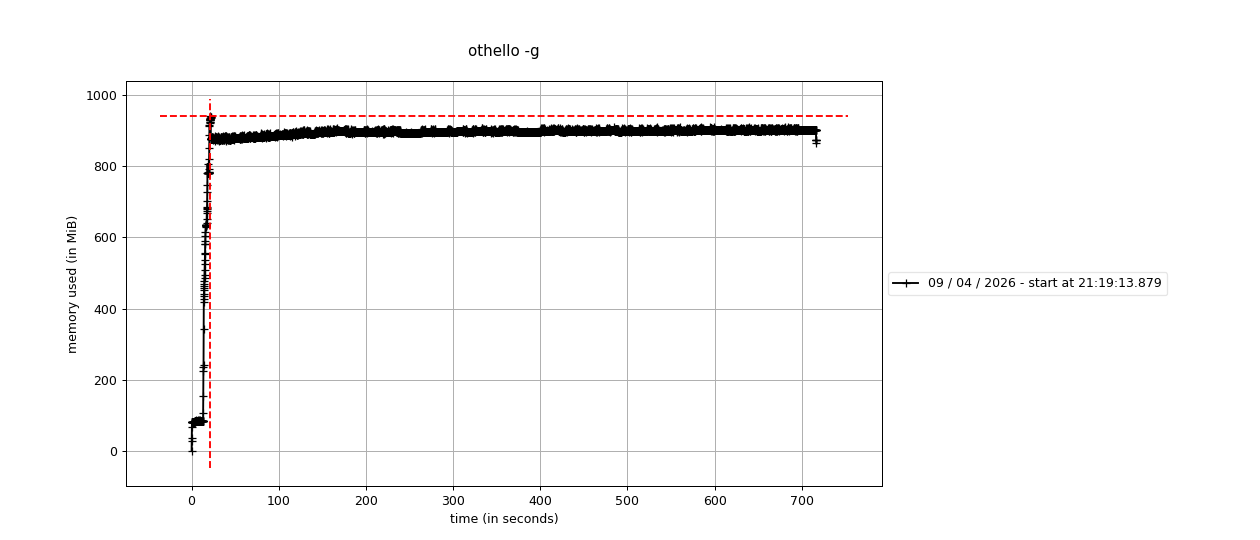
\includegraphics[width=0.85\textwidth]{images/conso_ram_MCTS_DL_12x12.png}
    \caption{Évolution de l'allocation mémoire.}
    \label{fig:mem_alloc}
    
    \vspace{0.5cm} 
    
    
    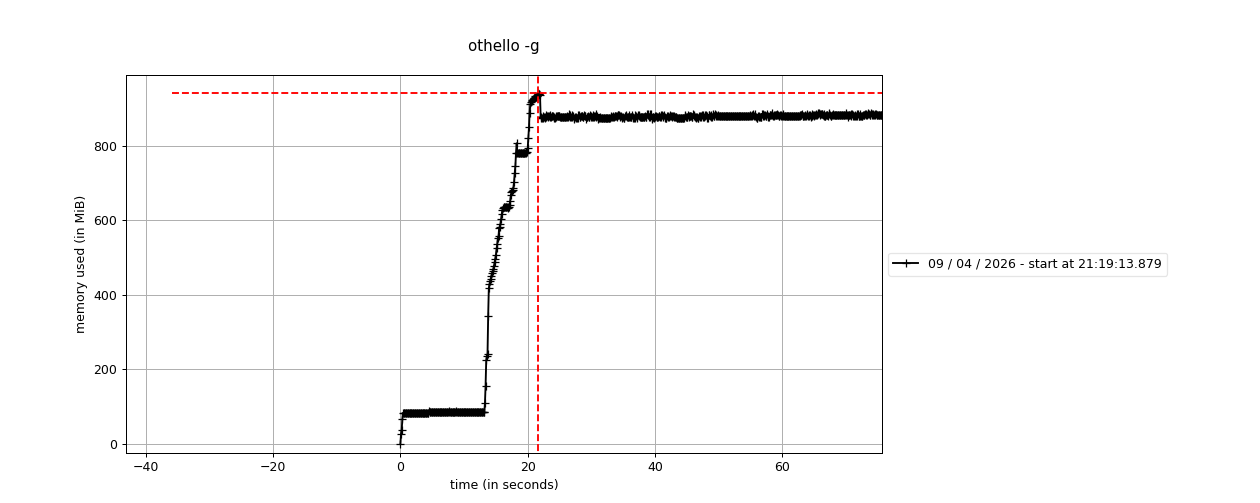
\includegraphics[width=0.85\textwidth]{images/conso_ram_MCTS_DL_12x12_zoom.png}
    \caption{Zoom sur l'apogée de la mémoire.}
    \label{fig:mem_oom}
    
\end{figure}

L'\textbf{incompatibilité OS du mode démon} notamment avec utilisation de \texttt{os.fork()} dans \texttt{app\_orchestrator.py} pour lancer le serveur en arrière-plan (mode démon) est une fonctionnalité spécifique aux systèmes POSIX. 
Ce choix architectural lie fortement le programme à GNU/Linux (ce qui respecte techniquement l'exigence \textbf{F1.5}) mais introduit des vulnérabilités de portabilité si le projet devait être compilé ou distribué sur des environnements Windows.

Nous avons découvert une\textbf{faille logique dans le système d'invitations (Usurpation d'identité)}.Un bug inattendu a été identifié dans la gestion réseau des joueurs. 
Le scénario est le suivant : un joueur A invite un joueur B. Pendant que l'invitation est en attente, le joueur B change son nom, 
et le joueur A en profite pour se renommer avec l'ancien nom du joueur B.
À ce moment-là, le système permet au joueur A d'accepter l'invitation qu'il a lui-même envoyée. 
Ce défaut de logique s'explique par le fait que le serveur résout probablement les cibles des invitations via le pseudonyme courant (qui est mutable) 
plutôt que par un identifiant de session unique et immuable (comme un UUID ou l'ID de la \textit{socket}).

Un point négatif de notre projet est l'utilisation de nombreuses \textbf{dépendances système}.L'utilisation de \texttt{PyGObject} (GTK3) pour l'interface graphique rend le déploiement complexe, 
particulièrement sous Windows ou macOS. 
Cela nécessite l'installation de bibliothèques système tierces (\texttt{gir1.2-gtk-3.0}, \texttt{libcairo}), 
contrairement à des alternatives natives purement Python. 
De même dans la partie IA avec le choix des verions de TensorFlow et Scikit-learn, 
qui peuvent poser des problèmes de compatibilité selon les versions de Python et les systèmes d'exploitation.

\subsection{Améliorations possibles et Perspectives}

Afin d'ameliorer notre projet, nous avons identifié plusieurs axes d'amélioration possibles, 
notamment pour renforcer la portabilité et les performances de notre jeu Othello.

Une des premières améliorations serait de \textbf{Migration vers GTK4}, mettre à jour le framework GUI via PyGObject pour utiliser \texttt{Gtk 4.0}. 
Cela permettrait de bénéficier d'API modernes pour implémenter de manière native et fluide le système de Glisser-Déposer (\textbf{F30}). 
De plus, GTK4 offre une meilleure gestion de la VRAM et des performances graphiques, ce qui améliorerait la réactivité de l'interface.
Un autre point d'amélioration serait l'\textbf{inférence par lots (Batched Prediction) pour le MCTS}. Au lieu de soumettre les nœuds unitairement au modèle Keras, 
l'arbre MCTS devrait être refactorisé pour accumuler les états à évaluer et les soumettre sous forme de \textit{batch} matriciel (ex: par blocs de 64). 
L'utilisation de la vectorisation de TensorFlow multiplierait de façon exponentielle les performances de la fonction de sélection.
Nous pourrions aussi utiliser les \textbf{tables de Transposition (Zobrist Hashing)}. Dans l'algorithme Negamax actuel, 
des plateaux strictement identiques (atteints par des séquences de coups différentes) sont réévalués inutilement. 
Ajouter une fonction de hachage sur 64-bits pour mémoriser les résultats intermédiaires dans un dictionnaire réduirait considérablement le facteur de branchement de l'arbre.
Nous avons aussi penser à faire une \textbf{Refonte du Serveur en mode Asynchrone}.
Remplacer l'architecture réseau basée sur la création de processus (\texttt{os.fork}) par une approche asynchrone utilisant la bibliothèque standard \texttt{asyncio}. 
Cette évolution fiabilisera la tenue en charge des connexions TCP multiples et simplifiera l'implémentation de la machine à états requise pour le complexe système 
d'invitations et de \textit{timeouts} (\textbf{F40}).
Actuellement il n'y pas d'animations sur les pions, nous pourrions ajouter des \textbf{Animations et des retours visuels (GUI)}.Actuellement, les pions changent de couleur instantanément. 
L'ajout de transitions CSS fluides pour le retournement des pions ou la mise en surbrillance du dernier coup joué par l'adversaire améliorerait
 l'expérience visuelle du joueur humain.
Enfin comme derniere amélioration, nous envisagions l'\textbf{intégration native de \texttt{asyncio} pour GTK}. Remplacer l'usage des \texttt{queue.Queue} 
et des threads classiques par la boucle d'événements asynchrone de GTK (via des adaptateurs). 
Cela simplifierait la communication réseau-GUI sans maintenir de boucles d'attente actives (\textit{polling}) dans l'orchestrateur.


\section{L'utilisation de l'Intelligence Artificielle dans notre projet}

Dans le cadre de ce projet, nous avons utilisé l'Intelligence Artificielle notamment des LLM (Large Language Models) pour nous aider dans le développement du logiciel.
Cela nous a permis d'automatiser les tâches chronophages pour nous concentrer sur l'architecture, la logique métier et l'apprentissage.

\subsection{Modèles exploités et Cas d'usage}
Nous avons jonglé entre plusieurs modèles selon nos besoins :
\begin{itemize}
    \item \textbf{Gemini 3.0 et Gemini 3.1 :} Ce sont les modèles que nous avons le plus utilisés au quotidien. Ils sont très rapides et ont été parfaits pour générer des tests répétitifs, nous expliquer des concepts de cours ou corriger des petits bugs.
    \item \textbf{Claude Sonnet 4.5 :} Nous l'avons surtout utilisé quand nous avions de gros bugs, où des questions complexes. Ce modèle est très doué pour structurer le code proprement et il explique son raisonnement de manière très pédagogique.
    \item \textbf{Deepseek et Qwen :} Nous les avons gardés comme alternatives. Quand on bloquait complètement sur un algorithme spécifique ou qu'on n'arrivait pas à obtenir une bonne réponse avec les autres IA, on leur posait la question pour avoir une approche différente. Mais aussi par curiosité pour comparer les réponses de différents modèles.
    \item \textbf{Ollama Model OpenSource :} Nous l'avons utilisé comme une alternative open-source pour tester des fonctionnalités spécifiques ou pour éviter les limitations des modèles propriétaires et par curiosité de voir ce que les modèles open-source pouvaient faire.
\end{itemize}

Nous avons utilisé l'IA pour faire des
\textbf{Tests automatisés}  avec la génération de la structure des tests et identification de cas limites, avec une validation humaine systématique.
De plus dans le cadre de l'\textbf{Apprentissage et débuggage} pour mieux comprendre de nouvelles bibliothèques via des exemples et identification d'erreurs de syntaxe ou de logique lors de blocages.
Mais aussi pour la \textbf{documentation } pour la génération des commentaires, du \texttt{README.md} et de la documentation technique à partir de notre code finalisé et fonctionnel.

\subsection{Cadre éthique et Bilan}
Conscients des risques d'« hallucinations », nous avons imposé une règle stricte : chaque ligne de code suggérée devait être lue, comprise et testée avant intégration. L'équipe assume l'entière responsabilité de l'architecture et du code final. 

En définitive, l'utilisation de l'IA a agi comme un tuteur et un développeur expérimenté pour nous aider à la réalisation du projet. Son utilisation critique et raisonnée a non seulement amélioré la qualité de notre code (tests, documentation, propreté du code), mais a aussi enrichi notre apprentissage technique et notre gestion de projet.


\section*{Conclusion}

Ce projet de développement d'un jeu d'Othello a été un défi technique qui a abouti à une application modulaire, intégrant des interfaces variées (GUI/CLI), 
un moteur de jeu optimisé par des \textit{Bitboards}, un serveur multijoueur multithreadé avec une bonne gestion des erreurs(déconnexion, latence, etc...) et une partie Intelligence Artificielle adaptée aux besoins du jeu Othello.
L'architecture logicielle, inspirée du modèle MVC, a permis un développement collaboratif efficace et une implémentation fluide de fonctionnalités avancées. 
Pour la partie Intelligence Artificielle, l'implementation des fonctions a révélé que sous la contrainte du temps réel, la rapidité d'exploration arborescente des algorithmes classiques (Négamax) 
surpasse la qualité d'évaluation unitaire des modèles d'apprentissage (Machine et Deep Learning via MCTS) freinés par leur latence. 
De plus avec l'utilisation d'IA générative comme outil d'assistance de développement, cela nous a permis de livrer un logiciel respectant le cahier des charges \cite{OthelloSpecs2025}, 
tout en adaptant un regard critique sur nos choix d'implementations (limites de Python et de la portabilité POSIX) pour identifier des pistes d'amélioration avec l'utilisation de \texttt{asyncio} ou GTK4.

%------------------------------------------------------------------------------
% BIBLIOGRAPHY
%------------------------------------------------------------------------------

\nocite{*}
\bibliographystyle{plain}
\bibliography{bibliography}

%------------------------------------------------------------------------------
% BACK MATTER
%------------------------------------------------------------------------------
\newpage
\appendix

\section{Annexe : Liste des Besoins}
\begin{itemize}
    \item F1. Lancement du programme : Fait
    \item F2. Fichier de configuration : Fait
    \item F3. Internationalisation (i18n) : Fait
    \item F4. Interface en ligne de commande : Fait
    \item F5. Mode blitz : Fait
    \item F6. Mode contest : Fait
    \item F7. Interface graphique : Fait
    \item F8. Mode IA : Fait
    \item F9. Taille du plateau : Fait
    \item F10. Gestion des règles : Fait
    \item F11. Gestion des erreurs de l'utilisateur : Fait
    \item F12. Gestion du undo/redo : Fait
    \item F13. Gestion des conseils : Fait
    \item F14. Gestion du blitz : Fait
    \item F15. Shell interactif : Fait
    \item F16. Proposer de sauvegarder avant de quitter : Fait
    \item F17. Édition de la commande en cours : Fait
    \item F18. Historique des commandes tapées : Fait
    \item F19. Complétion des commandes : Fait
    \item F20. Notation des coups : Fait
    \item F21. Sauvegarde et restauration d'une partie : Fait
    \item F22. Commentaires dans la sauvegarde : Fait
    \item F23. Format des paramètres du jeu : Fait
    \item F24. Format du plateau de jeu : Fait
    \item F25. Format de l'historique : Fait
    \item F26. Module bitboard : Fait
    \item F27. Algorithmes de manipulation des bitboards : Fait
    \item F28. Menus de l'application : Fait
    \item F29. Raccourcis clavier : Fait
    \item F30. Drag'n'Drop : Fait
    \item F31. Temps de réflexion borné : Fait
    \item F32. Minimax avec aß-pruning : Fait
    \item F33. Fonctions d'évaluation pour Minimax : Fait
    \item F34. Approfondissement itératif de Minimax : Fait
    \item F35. Profondeur de recherche de Minimax : Fait
    \item F36. Monte Carlo Tree Search (MCTS) : Fait
    \item F37. Fonction de sélection par Machine Learning : Fait
    \item F38. Découverte de serveurs et connexion client-serveur basique : Partiel (bug historique des commandes quand en attente de coup/au lobby/autocompletion aussi)
    \item F39. Serveur multi-clients et gestion de parties : Fait
    \item F40. Système d'invitations et gestion avancée des joueurs : Fait
\end{itemize}
\end{document}